% Created by tikzDevice version 0.12.4 on 2023-09-10 18:37:24
% !TEX encoding = UTF-8 Unicode
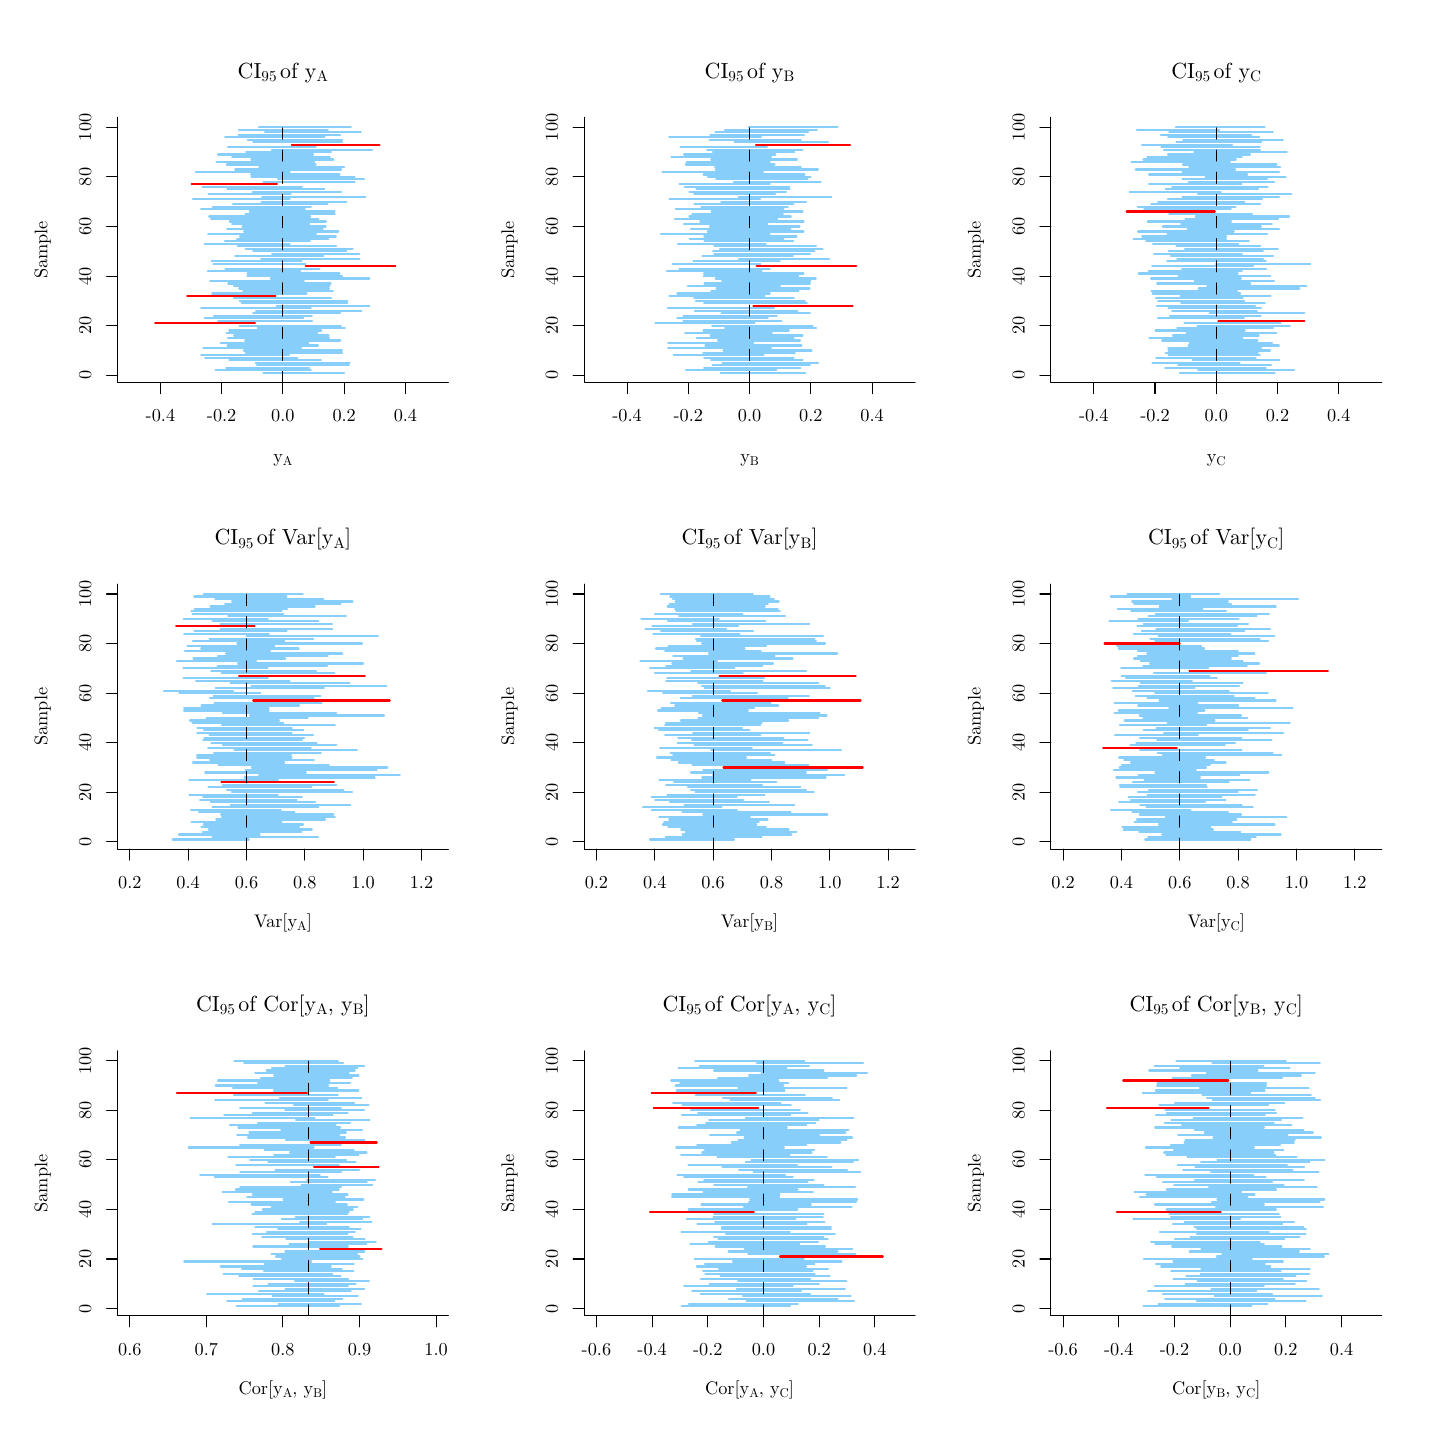
\begin{tikzpicture}[x=1pt,y=1pt]
\definecolor{fillColor}{RGB}{255,255,255}
\path[use as bounding box,fill=fillColor,fill opacity=0.00] (0,0) rectangle (505.89,505.89);
\begin{scope}
\path[clip] ( 32.47,377.65) rectangle (152.00,473.42);
\definecolor{drawColor}{RGB}{0,0,0}

\path[draw=drawColor,line width= 0.4pt,line join=round,line cap=round] (202.91,371.35) circle (  1.49);
\end{scope}
\begin{scope}
\path[clip] (  0.00,  0.00) rectangle (505.89,505.89);
\definecolor{drawColor}{RGB}{0,0,0}

\path[draw=drawColor,line width= 0.4pt,line join=round,line cap=round] ( 47.97,377.65) -- (136.50,377.65);

\path[draw=drawColor,line width= 0.4pt,line join=round,line cap=round] ( 47.97,377.65) -- ( 47.97,373.69);

\path[draw=drawColor,line width= 0.4pt,line join=round,line cap=round] ( 70.10,377.65) -- ( 70.10,373.69);

\path[draw=drawColor,line width= 0.4pt,line join=round,line cap=round] ( 92.23,377.65) -- ( 92.23,373.69);

\path[draw=drawColor,line width= 0.4pt,line join=round,line cap=round] (114.37,377.65) -- (114.37,373.69);

\path[draw=drawColor,line width= 0.4pt,line join=round,line cap=round] (136.50,377.65) -- (136.50,373.69);

\node[text=drawColor,anchor=base,inner sep=0pt, outer sep=0pt, scale=  0.66] at ( 47.97,363.40) {-0.4};

\node[text=drawColor,anchor=base,inner sep=0pt, outer sep=0pt, scale=  0.66] at ( 70.10,363.40) {-0.2};

\node[text=drawColor,anchor=base,inner sep=0pt, outer sep=0pt, scale=  0.66] at ( 92.23,363.40) {0.0};

\node[text=drawColor,anchor=base,inner sep=0pt, outer sep=0pt, scale=  0.66] at (114.37,363.40) {0.2};

\node[text=drawColor,anchor=base,inner sep=0pt, outer sep=0pt, scale=  0.66] at (136.50,363.40) {0.4};

\path[draw=drawColor,line width= 0.4pt,line join=round,line cap=round] ( 32.47,380.30) -- ( 32.47,469.87);

\path[draw=drawColor,line width= 0.4pt,line join=round,line cap=round] ( 32.47,380.30) -- ( 28.51,380.30);

\path[draw=drawColor,line width= 0.4pt,line join=round,line cap=round] ( 32.47,398.22) -- ( 28.51,398.22);

\path[draw=drawColor,line width= 0.4pt,line join=round,line cap=round] ( 32.47,416.13) -- ( 28.51,416.13);

\path[draw=drawColor,line width= 0.4pt,line join=round,line cap=round] ( 32.47,434.04) -- ( 28.51,434.04);

\path[draw=drawColor,line width= 0.4pt,line join=round,line cap=round] ( 32.47,451.96) -- ( 28.51,451.96);

\path[draw=drawColor,line width= 0.4pt,line join=round,line cap=round] ( 32.47,469.87) -- ( 28.51,469.87);

\node[text=drawColor,rotate= 90.00,anchor=base,inner sep=0pt, outer sep=0pt, scale=  0.66] at ( 22.97,380.30) {0};

\node[text=drawColor,rotate= 90.00,anchor=base,inner sep=0pt, outer sep=0pt, scale=  0.66] at ( 22.97,398.22) {20};

\node[text=drawColor,rotate= 90.00,anchor=base,inner sep=0pt, outer sep=0pt, scale=  0.66] at ( 22.97,416.13) {40};

\node[text=drawColor,rotate= 90.00,anchor=base,inner sep=0pt, outer sep=0pt, scale=  0.66] at ( 22.97,434.04) {60};

\node[text=drawColor,rotate= 90.00,anchor=base,inner sep=0pt, outer sep=0pt, scale=  0.66] at ( 22.97,451.96) {80};

\node[text=drawColor,rotate= 90.00,anchor=base,inner sep=0pt, outer sep=0pt, scale=  0.66] at ( 22.97,469.87) {100};

\path[draw=drawColor,line width= 0.4pt,line join=round,line cap=round] ( 32.47,473.42) --
	( 32.47,377.65) --
	(152.00,377.65);
\end{scope}
\begin{scope}
\path[clip] (  0.00,337.26) rectangle (168.63,505.89);
\definecolor{drawColor}{RGB}{0,0,0}

\node[text=drawColor,anchor=base west,inner sep=0pt, outer sep=0pt, scale=  0.79] at ( 75.90,487.67) {CI};

\node[text=drawColor,anchor=base west,inner sep=0pt, outer sep=0pt, scale=  0.55] at ( 84.48,486.48) {95};

\node[text=drawColor,anchor=base west,inner sep=0pt, outer sep=0pt, scale=  0.79] at ( 90.02,487.67) {\hspace{1.5pt}of y};

\node[text=drawColor,anchor=base west,inner sep=0pt, outer sep=0pt, scale=  0.55] at (104.41,486.48) {A};

\node[text=drawColor,anchor=base west,inner sep=0pt, outer sep=0pt, scale=  0.66] at ( 88.76,348.84) {y};

\node[text=drawColor,anchor=base west,inner sep=0pt, outer sep=0pt, scale=  0.46] at ( 92.24,347.84) {A};

\node[text=drawColor,rotate= 90.00,anchor=base,inner sep=0pt, outer sep=0pt, scale=  0.66] at (  7.13,425.53) {Sample};
\end{scope}
\begin{scope}
\path[clip] ( 32.47,377.65) rectangle (152.00,473.42);
\definecolor{drawColor}{RGB}{135,206,250}

\path[draw=drawColor,line width= 0.8pt,line join=round,line cap=round] ( 85.22,381.20) --
	(114.33,381.20);

\path[draw=drawColor,line width= 0.8pt,line join=round,line cap=round] ( 67.93,382.09) --
	(102.27,382.09);

\path[draw=drawColor,line width= 0.8pt,line join=round,line cap=round] ( 71.71,382.99) --
	(101.71,382.99);

\path[draw=drawColor,line width= 0.8pt,line join=round,line cap=round] ( 82.85,383.89) --
	(116.01,383.89);

\path[draw=drawColor,line width= 0.8pt,line join=round,line cap=round] ( 82.39,384.78) --
	(116.29,384.78);

\path[draw=drawColor,line width= 0.8pt,line join=round,line cap=round] ( 72.95,385.68) --
	(105.95,385.68);

\path[draw=drawColor,line width= 0.8pt,line join=round,line cap=round] ( 64.13,386.57) --
	( 97.40,386.57);

\path[draw=drawColor,line width= 0.8pt,line join=round,line cap=round] ( 62.74,387.47) --
	( 94.44,387.47);

\path[draw=drawColor,line width= 0.8pt,line join=round,line cap=round] ( 78.81,388.36) --
	(113.63,388.36);

\path[draw=drawColor,line width= 0.8pt,line join=round,line cap=round] ( 78.10,389.26) --
	(113.59,389.26);

\path[draw=drawColor,line width= 0.8pt,line join=round,line cap=round] ( 63.42,390.16) --
	( 98.81,390.16);

\path[draw=drawColor,line width= 0.8pt,line join=round,line cap=round] ( 72.24,391.05) --
	(104.89,391.05);

\path[draw=drawColor,line width= 0.8pt,line join=round,line cap=round] ( 69.76,391.95) --
	(101.40,391.95);

\path[draw=drawColor,line width= 0.8pt,line join=round,line cap=round] ( 78.57,392.84) --
	(112.93,392.84);

\path[draw=drawColor,line width= 0.8pt,line join=round,line cap=round] ( 72.38,393.74) --
	(108.90,393.74);

\path[draw=drawColor,line width= 0.8pt,line join=round,line cap=round] ( 74.59,394.63) --
	(108.72,394.63);

\path[draw=drawColor,line width= 0.8pt,line join=round,line cap=round] ( 71.86,395.53) --
	(104.67,395.53);

\path[draw=drawColor,line width= 0.8pt,line join=round,line cap=round] ( 72.86,396.43) --
	(106.05,396.43);

\path[draw=drawColor,line width= 0.8pt,line join=round,line cap=round] ( 83.14,397.32) --
	(114.56,397.32);

\path[draw=drawColor,line width= 0.8pt,line join=round,line cap=round] ( 76.55,398.22) --
	(113.19,398.22);
\definecolor{drawColor}{RGB}{255,0,0}

\path[draw=drawColor,line width= 0.8pt,line join=round,line cap=round] ( 46.07,399.11) --
	( 82.13,399.11);
\definecolor{drawColor}{RGB}{135,206,250}

\path[draw=drawColor,line width= 0.8pt,line join=round,line cap=round] ( 68.86,400.01) --
	(102.74,400.01);

\path[draw=drawColor,line width= 0.8pt,line join=round,line cap=round] ( 63.98,400.90) --
	( 99.57,400.90);

\path[draw=drawColor,line width= 0.8pt,line join=round,line cap=round] ( 67.29,401.80) --
	(102.71,401.80);

\path[draw=drawColor,line width= 0.8pt,line join=round,line cap=round] ( 81.47,402.70) --
	(112.88,402.70);

\path[draw=drawColor,line width= 0.8pt,line join=round,line cap=round] ( 82.52,403.59) --
	(120.59,403.59);

\path[draw=drawColor,line width= 0.8pt,line join=round,line cap=round] ( 62.69,404.49) --
	(102.31,404.49);

\path[draw=drawColor,line width= 0.8pt,line join=round,line cap=round] ( 90.01,405.38) --
	(123.47,405.38);

\path[draw=drawColor,line width= 0.8pt,line join=round,line cap=round] ( 77.31,406.28) --
	(115.51,406.28);

\path[draw=drawColor,line width= 0.8pt,line join=round,line cap=round] ( 76.61,407.17) --
	(115.47,407.17);

\path[draw=drawColor,line width= 0.8pt,line join=round,line cap=round] ( 74.53,408.07) --
	(109.60,408.07);
\definecolor{drawColor}{RGB}{255,0,0}

\path[draw=drawColor,line width= 0.8pt,line join=round,line cap=round] ( 57.61,408.96) --
	( 89.50,408.96);
\definecolor{drawColor}{RGB}{135,206,250}

\path[draw=drawColor,line width= 0.8pt,line join=round,line cap=round] ( 66.70,409.86) --
	(100.77,409.86);

\path[draw=drawColor,line width= 0.8pt,line join=round,line cap=round] ( 77.87,410.76) --
	(110.31,410.76);

\path[draw=drawColor,line width= 0.8pt,line join=round,line cap=round] ( 76.43,411.65) --
	(108.83,411.65);

\path[draw=drawColor,line width= 0.8pt,line join=round,line cap=round] ( 74.54,412.55) --
	(109.07,412.55);

\path[draw=drawColor,line width= 0.8pt,line join=round,line cap=round] ( 72.50,413.44) --
	(109.45,413.44);

\path[draw=drawColor,line width= 0.8pt,line join=round,line cap=round] ( 65.98,414.34) --
	( 99.81,414.34);

\path[draw=drawColor,line width= 0.8pt,line join=round,line cap=round] ( 87.84,415.23) --
	(123.42,415.23);

\path[draw=drawColor,line width= 0.8pt,line join=round,line cap=round] ( 79.38,416.13) --
	(113.61,416.13);

\path[draw=drawColor,line width= 0.8pt,line join=round,line cap=round] ( 79.45,417.03) --
	(112.65,417.03);

\path[draw=drawColor,line width= 0.8pt,line join=round,line cap=round] ( 65.13,417.92) --
	( 98.49,417.92);

\path[draw=drawColor,line width= 0.8pt,line join=round,line cap=round] ( 71.49,418.82) --
	(105.48,418.82);
\definecolor{drawColor}{RGB}{255,0,0}

\path[draw=drawColor,line width= 0.8pt,line join=round,line cap=round] (100.43,419.71) --
	(132.87,419.71);
\definecolor{drawColor}{RGB}{135,206,250}

\path[draw=drawColor,line width= 0.8pt,line join=round,line cap=round] ( 67.09,420.61) --
	(100.38,420.61);

\path[draw=drawColor,line width= 0.8pt,line join=round,line cap=round] ( 66.51,421.50) --
	( 98.97,421.50);

\path[draw=drawColor,line width= 0.8pt,line join=round,line cap=round] ( 84.41,422.40) --
	(119.91,422.40);

\path[draw=drawColor,line width= 0.8pt,line join=round,line cap=round] ( 74.97,423.30) --
	(106.81,423.30);

\path[draw=drawColor,line width= 0.8pt,line join=round,line cap=round] ( 88.36,424.19) --
	(119.86,424.19);

\path[draw=drawColor,line width= 0.8pt,line join=round,line cap=round] ( 81.50,425.09) --
	(115.11,425.09);

\path[draw=drawColor,line width= 0.8pt,line join=round,line cap=round] ( 78.75,425.98) --
	(117.40,425.98);

\path[draw=drawColor,line width= 0.8pt,line join=round,line cap=round] ( 75.86,426.88) --
	(111.44,426.88);

\path[draw=drawColor,line width= 0.8pt,line join=round,line cap=round] ( 63.98,427.77) --
	( 94.68,427.77);

\path[draw=drawColor,line width= 0.8pt,line join=round,line cap=round] ( 71.29,428.67) --
	(102.00,428.67);

\path[draw=drawColor,line width= 0.8pt,line join=round,line cap=round] ( 75.64,429.57) --
	(108.63,429.57);

\path[draw=drawColor,line width= 0.8pt,line join=round,line cap=round] ( 76.76,430.46) --
	(111.35,430.46);

\path[draw=drawColor,line width= 0.8pt,line join=round,line cap=round] ( 65.20,431.36) --
	(104.21,431.36);

\path[draw=drawColor,line width= 0.8pt,line join=round,line cap=round] ( 78.17,432.25) --
	(112.20,432.25);

\path[draw=drawColor,line width= 0.8pt,line join=round,line cap=round] ( 72.10,433.15) --
	(106.60,433.15);

\path[draw=drawColor,line width= 0.8pt,line join=round,line cap=round] ( 77.61,434.04) --
	(107.66,434.04);

\path[draw=drawColor,line width= 0.8pt,line join=round,line cap=round] ( 73.90,434.94) --
	(101.71,434.94);

\path[draw=drawColor,line width= 0.8pt,line join=round,line cap=round] ( 73.01,435.84) --
	(107.74,435.84);

\path[draw=drawColor,line width= 0.8pt,line join=round,line cap=round] ( 66.27,436.73) --
	(105.07,436.73);

\path[draw=drawColor,line width= 0.8pt,line join=round,line cap=round] ( 65.61,437.63) --
	(102.08,437.63);

\path[draw=drawColor,line width= 0.8pt,line join=round,line cap=round] ( 78.70,438.52) --
	(110.99,438.52);

\path[draw=drawColor,line width= 0.8pt,line join=round,line cap=round] ( 80.22,439.42) --
	(110.86,439.42);

\path[draw=drawColor,line width= 0.8pt,line join=round,line cap=round] ( 62.65,440.31) --
	(100.10,440.31);

\path[draw=drawColor,line width= 0.8pt,line join=round,line cap=round] ( 66.89,441.21) --
	(102.34,441.21);

\path[draw=drawColor,line width= 0.8pt,line join=round,line cap=round] ( 74.15,442.11) --
	(108.35,442.11);

\path[draw=drawColor,line width= 0.8pt,line join=round,line cap=round] ( 84.49,443.00) --
	(115.11,443.00);

\path[draw=drawColor,line width= 0.8pt,line join=round,line cap=round] ( 59.73,443.90) --
	( 94.68,443.90);

\path[draw=drawColor,line width= 0.8pt,line join=round,line cap=round] ( 84.69,444.79) --
	(122.03,444.79);

\path[draw=drawColor,line width= 0.8pt,line join=round,line cap=round] ( 65.33,445.69) --
	( 95.04,445.69);

\path[draw=drawColor,line width= 0.8pt,line join=round,line cap=round] ( 81.25,446.58) --
	(113.22,446.58);

\path[draw=drawColor,line width= 0.8pt,line join=round,line cap=round] ( 72.18,447.48) --
	(107.19,447.48);

\path[draw=drawColor,line width= 0.8pt,line join=round,line cap=round] ( 63.13,448.37) --
	( 99.11,448.37);
\definecolor{drawColor}{RGB}{255,0,0}

\path[draw=drawColor,line width= 0.8pt,line join=round,line cap=round] ( 59.26,449.27) --
	( 90.08,449.27);
\definecolor{drawColor}{RGB}{135,206,250}

\path[draw=drawColor,line width= 0.8pt,line join=round,line cap=round] ( 85.19,450.17) --
	(118.15,450.17);

\path[draw=drawColor,line width= 0.8pt,line join=round,line cap=round] ( 90.38,451.06) --
	(121.53,451.06);

\path[draw=drawColor,line width= 0.8pt,line join=round,line cap=round] ( 80.85,451.96) --
	(118.12,451.96);

\path[draw=drawColor,line width= 0.8pt,line join=round,line cap=round] ( 80.74,452.85) --
	(112.64,452.85);

\path[draw=drawColor,line width= 0.8pt,line join=round,line cap=round] ( 60.68,453.75) --
	( 94.68,453.75);

\path[draw=drawColor,line width= 0.8pt,line join=round,line cap=round] ( 74.99,454.64) --
	(113.26,454.64);

\path[draw=drawColor,line width= 0.8pt,line join=round,line cap=round] ( 83.63,455.54) --
	(114.35,455.54);

\path[draw=drawColor,line width= 0.8pt,line join=round,line cap=round] ( 71.96,456.44) --
	(104.04,456.44);

\path[draw=drawColor,line width= 0.8pt,line join=round,line cap=round] ( 68.23,457.33) --
	(103.54,457.33);

\path[draw=drawColor,line width= 0.8pt,line join=round,line cap=round] ( 80.83,458.23) --
	(110.43,458.23);

\path[draw=drawColor,line width= 0.8pt,line join=round,line cap=round] ( 73.87,459.12) --
	(109.17,459.12);

\path[draw=drawColor,line width= 0.8pt,line join=round,line cap=round] ( 68.77,460.02) --
	(103.13,460.02);

\path[draw=drawColor,line width= 0.8pt,line join=round,line cap=round] ( 78.92,460.91) --
	(109.56,460.91);

\path[draw=drawColor,line width= 0.8pt,line join=round,line cap=round] ( 88.21,461.81) --
	(124.43,461.81);

\path[draw=drawColor,line width= 0.8pt,line join=round,line cap=round] ( 72.32,462.71) --
	(104.15,462.71);
\definecolor{drawColor}{RGB}{255,0,0}

\path[draw=drawColor,line width= 0.8pt,line join=round,line cap=round] ( 95.43,463.60) --
	(127.12,463.60);
\definecolor{drawColor}{RGB}{135,206,250}

\path[draw=drawColor,line width= 0.8pt,line join=round,line cap=round] ( 81.48,464.50) --
	(113.59,464.50);

\path[draw=drawColor,line width= 0.8pt,line join=round,line cap=round] ( 79.54,465.39) --
	(113.64,465.39);

\path[draw=drawColor,line width= 0.8pt,line join=round,line cap=round] ( 71.37,466.29) --
	(107.25,466.29);

\path[draw=drawColor,line width= 0.8pt,line join=round,line cap=round] ( 76.21,467.18) --
	(112.87,467.18);

\path[draw=drawColor,line width= 0.8pt,line join=round,line cap=round] ( 85.69,468.08) --
	(120.39,468.08);

\path[draw=drawColor,line width= 0.8pt,line join=round,line cap=round] ( 76.35,468.98) --
	(108.42,468.98);

\path[draw=drawColor,line width= 0.8pt,line join=round,line cap=round] ( 83.52,469.87) --
	(116.79,469.87);
\definecolor{drawColor}{RGB}{0,0,0}

\path[draw=drawColor,line width= 0.4pt,dash pattern=on 4pt off 4pt ,line join=round,line cap=round] ( 92.23,377.65) -- ( 92.23,473.42);
\end{scope}
\begin{scope}
\path[clip] (201.10,377.65) rectangle (320.63,473.42);
\definecolor{drawColor}{RGB}{0,0,0}

\path[draw=drawColor,line width= 0.4pt,line join=round,line cap=round] (371.54,371.35) circle (  1.49);
\end{scope}
\begin{scope}
\path[clip] (  0.00,  0.00) rectangle (505.89,505.89);
\definecolor{drawColor}{RGB}{0,0,0}

\path[draw=drawColor,line width= 0.4pt,line join=round,line cap=round] (216.60,377.65) -- (305.13,377.65);

\path[draw=drawColor,line width= 0.4pt,line join=round,line cap=round] (216.60,377.65) -- (216.60,373.69);

\path[draw=drawColor,line width= 0.4pt,line join=round,line cap=round] (238.73,377.65) -- (238.73,373.69);

\path[draw=drawColor,line width= 0.4pt,line join=round,line cap=round] (260.87,377.65) -- (260.87,373.69);

\path[draw=drawColor,line width= 0.4pt,line join=round,line cap=round] (283.00,377.65) -- (283.00,373.69);

\path[draw=drawColor,line width= 0.4pt,line join=round,line cap=round] (305.13,377.65) -- (305.13,373.69);

\node[text=drawColor,anchor=base,inner sep=0pt, outer sep=0pt, scale=  0.66] at (216.60,363.40) {-0.4};

\node[text=drawColor,anchor=base,inner sep=0pt, outer sep=0pt, scale=  0.66] at (238.73,363.40) {-0.2};

\node[text=drawColor,anchor=base,inner sep=0pt, outer sep=0pt, scale=  0.66] at (260.87,363.40) {0.0};

\node[text=drawColor,anchor=base,inner sep=0pt, outer sep=0pt, scale=  0.66] at (283.00,363.40) {0.2};

\node[text=drawColor,anchor=base,inner sep=0pt, outer sep=0pt, scale=  0.66] at (305.13,363.40) {0.4};

\path[draw=drawColor,line width= 0.4pt,line join=round,line cap=round] (201.10,380.30) -- (201.10,469.87);

\path[draw=drawColor,line width= 0.4pt,line join=round,line cap=round] (201.10,380.30) -- (197.14,380.30);

\path[draw=drawColor,line width= 0.4pt,line join=round,line cap=round] (201.10,398.22) -- (197.14,398.22);

\path[draw=drawColor,line width= 0.4pt,line join=round,line cap=round] (201.10,416.13) -- (197.14,416.13);

\path[draw=drawColor,line width= 0.4pt,line join=round,line cap=round] (201.10,434.04) -- (197.14,434.04);

\path[draw=drawColor,line width= 0.4pt,line join=round,line cap=round] (201.10,451.96) -- (197.14,451.96);

\path[draw=drawColor,line width= 0.4pt,line join=round,line cap=round] (201.10,469.87) -- (197.14,469.87);

\node[text=drawColor,rotate= 90.00,anchor=base,inner sep=0pt, outer sep=0pt, scale=  0.66] at (191.60,380.30) {0};

\node[text=drawColor,rotate= 90.00,anchor=base,inner sep=0pt, outer sep=0pt, scale=  0.66] at (191.60,398.22) {20};

\node[text=drawColor,rotate= 90.00,anchor=base,inner sep=0pt, outer sep=0pt, scale=  0.66] at (191.60,416.13) {40};

\node[text=drawColor,rotate= 90.00,anchor=base,inner sep=0pt, outer sep=0pt, scale=  0.66] at (191.60,434.04) {60};

\node[text=drawColor,rotate= 90.00,anchor=base,inner sep=0pt, outer sep=0pt, scale=  0.66] at (191.60,451.96) {80};

\node[text=drawColor,rotate= 90.00,anchor=base,inner sep=0pt, outer sep=0pt, scale=  0.66] at (191.60,469.87) {100};

\path[draw=drawColor,line width= 0.4pt,line join=round,line cap=round] (201.10,473.42) --
	(201.10,377.65) --
	(320.63,377.65);
\end{scope}
\begin{scope}
\path[clip] (168.63,337.26) rectangle (337.26,505.89);
\definecolor{drawColor}{RGB}{0,0,0}

\node[text=drawColor,anchor=base west,inner sep=0pt, outer sep=0pt, scale=  0.79] at (244.65,487.67) {CI};

\node[text=drawColor,anchor=base west,inner sep=0pt, outer sep=0pt, scale=  0.55] at (253.23,486.48) {95};

\node[text=drawColor,anchor=base west,inner sep=0pt, outer sep=0pt, scale=  0.79] at (258.77,487.67) {\hspace{1.5pt}of y};

\node[text=drawColor,anchor=base west,inner sep=0pt, outer sep=0pt, scale=  0.55] at (273.15,486.48) {B};

\node[text=drawColor,anchor=base west,inner sep=0pt, outer sep=0pt, scale=  0.66] at (257.49,348.84) {y};

\node[text=drawColor,anchor=base west,inner sep=0pt, outer sep=0pt, scale=  0.46] at (260.97,347.84) {B};

\node[text=drawColor,rotate= 90.00,anchor=base,inner sep=0pt, outer sep=0pt, scale=  0.66] at (175.76,425.53) {Sample};
\end{scope}
\begin{scope}
\path[clip] (201.10,377.65) rectangle (320.63,473.42);
\definecolor{drawColor}{RGB}{135,206,250}

\path[draw=drawColor,line width= 0.8pt,line join=round,line cap=round] (250.39,381.20) --
	(280.99,381.20);

\path[draw=drawColor,line width= 0.8pt,line join=round,line cap=round] (237.85,382.09) --
	(270.53,382.09);

\path[draw=drawColor,line width= 0.8pt,line join=round,line cap=round] (244.42,382.99) --
	(279.21,382.99);

\path[draw=drawColor,line width= 0.8pt,line join=round,line cap=round] (247.50,383.89) --
	(282.64,383.89);

\path[draw=drawColor,line width= 0.8pt,line join=round,line cap=round] (251.04,384.78) --
	(285.64,384.78);

\path[draw=drawColor,line width= 0.8pt,line join=round,line cap=round] (247.00,385.68) --
	(280.01,385.68);

\path[draw=drawColor,line width= 0.8pt,line join=round,line cap=round] (244.48,386.57) --
	(276.78,386.57);

\path[draw=drawColor,line width= 0.8pt,line join=round,line cap=round] (233.43,387.47) --
	(265.91,387.47);

\path[draw=drawColor,line width= 0.8pt,line join=round,line cap=round] (244.11,388.36) --
	(277.23,388.36);

\path[draw=drawColor,line width= 0.8pt,line join=round,line cap=round] (251.43,389.26) --
	(283.25,389.26);

\path[draw=drawColor,line width= 0.8pt,line join=round,line cap=round] (231.44,390.16) --
	(268.63,390.16);

\path[draw=drawColor,line width= 0.8pt,line join=round,line cap=round] (244.88,391.05) --
	(279.62,391.05);

\path[draw=drawColor,line width= 0.8pt,line join=round,line cap=round] (231.41,391.95) --
	(262.24,391.95);

\path[draw=drawColor,line width= 0.8pt,line join=round,line cap=round] (249.44,392.84) --
	(279.06,392.84);

\path[draw=drawColor,line width= 0.8pt,line join=round,line cap=round] (241.78,393.74) --
	(276.79,393.74);

\path[draw=drawColor,line width= 0.8pt,line join=round,line cap=round] (246.77,394.63) --
	(279.99,394.63);

\path[draw=drawColor,line width= 0.8pt,line join=round,line cap=round] (237.59,395.53) --
	(268.90,395.53);

\path[draw=drawColor,line width= 0.8pt,line join=round,line cap=round] (244.21,396.43) --
	(275.03,396.43);

\path[draw=drawColor,line width= 0.8pt,line join=round,line cap=round] (252.01,397.32) --
	(284.91,397.32);

\path[draw=drawColor,line width= 0.8pt,line join=round,line cap=round] (247.32,398.22) --
	(283.62,398.22);

\path[draw=drawColor,line width= 0.8pt,line join=round,line cap=round] (226.86,399.11) --
	(262.63,399.11);

\path[draw=drawColor,line width= 0.8pt,line join=round,line cap=round] (236.94,400.01) --
	(272.34,400.01);

\path[draw=drawColor,line width= 0.8pt,line join=round,line cap=round] (234.73,400.90) --
	(267.46,400.90);

\path[draw=drawColor,line width= 0.8pt,line join=round,line cap=round] (236.94,401.80) --
	(270.68,401.80);

\path[draw=drawColor,line width= 0.8pt,line join=round,line cap=round] (250.73,402.70) --
	(282.60,402.70);

\path[draw=drawColor,line width= 0.8pt,line join=round,line cap=round] (241.02,403.59) --
	(278.09,403.59);

\path[draw=drawColor,line width= 0.8pt,line join=round,line cap=round] (231.35,404.49) --
	(269.61,404.49);
\definecolor{drawColor}{RGB}{255,0,0}

\path[draw=drawColor,line width= 0.8pt,line join=round,line cap=round] (262.27,405.38) --
	(298.05,405.38);
\definecolor{drawColor}{RGB}{135,206,250}

\path[draw=drawColor,line width= 0.8pt,line join=round,line cap=round] (244.41,406.28) --
	(281.57,406.28);

\path[draw=drawColor,line width= 0.8pt,line join=round,line cap=round] (241.43,407.17) --
	(280.82,407.17);

\path[draw=drawColor,line width= 0.8pt,line join=round,line cap=round] (240.87,408.07) --
	(276.82,408.07);

\path[draw=drawColor,line width= 0.8pt,line join=round,line cap=round] (231.93,408.96) --
	(266.24,408.96);

\path[draw=drawColor,line width= 0.8pt,line join=round,line cap=round] (234.76,409.86) --
	(268.15,409.86);

\path[draw=drawColor,line width= 0.8pt,line join=round,line cap=round] (247.00,410.76) --
	(278.54,410.76);

\path[draw=drawColor,line width= 0.8pt,line join=round,line cap=round] (248.91,411.65) --
	(282.52,411.65);

\path[draw=drawColor,line width= 0.8pt,line join=round,line cap=round] (238.55,412.55) --
	(271.84,412.55);

\path[draw=drawColor,line width= 0.8pt,line join=round,line cap=round] (244.57,413.44) --
	(282.63,413.44);

\path[draw=drawColor,line width= 0.8pt,line join=round,line cap=round] (250.91,414.34) --
	(282.88,414.34);

\path[draw=drawColor,line width= 0.8pt,line join=round,line cap=round] (248.62,415.23) --
	(284.79,415.23);

\path[draw=drawColor,line width= 0.8pt,line join=round,line cap=round] (244.27,416.13) --
	(278.44,416.13);

\path[draw=drawColor,line width= 0.8pt,line join=round,line cap=round] (244.42,417.03) --
	(280.31,417.03);

\path[draw=drawColor,line width= 0.8pt,line join=round,line cap=round] (230.96,417.92) --
	(265.21,417.92);

\path[draw=drawColor,line width= 0.8pt,line join=round,line cap=round] (235.53,418.82) --
	(268.13,418.82);
\definecolor{drawColor}{RGB}{255,0,0}

\path[draw=drawColor,line width= 0.8pt,line join=round,line cap=round] (263.38,419.71) --
	(299.39,419.71);
\definecolor{drawColor}{RGB}{135,206,250}

\path[draw=drawColor,line width= 0.8pt,line join=round,line cap=round] (232.98,420.61) --
	(264.76,420.61);

\path[draw=drawColor,line width= 0.8pt,line join=round,line cap=round] (240.59,421.50) --
	(271.81,421.50);

\path[draw=drawColor,line width= 0.8pt,line join=round,line cap=round] (257.03,422.40) --
	(289.62,422.40);

\path[draw=drawColor,line width= 0.8pt,line join=round,line cap=round] (243.79,423.30) --
	(276.48,423.30);

\path[draw=drawColor,line width= 0.8pt,line join=round,line cap=round] (248.10,424.19) --
	(282.68,424.19);

\path[draw=drawColor,line width= 0.8pt,line join=round,line cap=round] (247.67,425.09) --
	(284.26,425.09);

\path[draw=drawColor,line width= 0.8pt,line join=round,line cap=round] (250.13,425.98) --
	(287.27,425.98);

\path[draw=drawColor,line width= 0.8pt,line join=round,line cap=round] (248.17,426.88) --
	(284.85,426.88);

\path[draw=drawColor,line width= 0.8pt,line join=round,line cap=round] (234.95,427.77) --
	(266.62,427.77);

\path[draw=drawColor,line width= 0.8pt,line join=round,line cap=round] (244.51,428.67) --
	(276.64,428.67);

\path[draw=drawColor,line width= 0.8pt,line join=round,line cap=round] (239.24,429.57) --
	(273.12,429.57);

\path[draw=drawColor,line width= 0.8pt,line join=round,line cap=round] (244.49,430.46) --
	(277.81,430.46);

\path[draw=drawColor,line width= 0.8pt,line join=round,line cap=round] (228.85,431.36) --
	(268.11,431.36);

\path[draw=drawColor,line width= 0.8pt,line join=round,line cap=round] (245.75,432.25) --
	(280.29,432.25);

\path[draw=drawColor,line width= 0.8pt,line join=round,line cap=round] (239.65,433.15) --
	(275.63,433.15);

\path[draw=drawColor,line width= 0.8pt,line join=round,line cap=round] (246.52,434.04) --
	(278.87,434.04);

\path[draw=drawColor,line width= 0.8pt,line join=round,line cap=round] (237.09,434.94) --
	(267.38,434.94);

\path[draw=drawColor,line width= 0.8pt,line join=round,line cap=round] (243.02,435.84) --
	(280.37,435.84);

\path[draw=drawColor,line width= 0.8pt,line join=round,line cap=round] (233.85,436.73) --
	(270.87,436.73);

\path[draw=drawColor,line width= 0.8pt,line join=round,line cap=round] (239.14,437.63) --
	(275.74,437.63);

\path[draw=drawColor,line width= 0.8pt,line join=round,line cap=round] (240.16,438.52) --
	(272.91,438.52);

\path[draw=drawColor,line width= 0.8pt,line join=round,line cap=round] (247.11,439.42) --
	(279.99,439.42);

\path[draw=drawColor,line width= 0.8pt,line join=round,line cap=round] (234.16,440.31) --
	(273.12,440.31);

\path[draw=drawColor,line width= 0.8pt,line join=round,line cap=round] (243.42,441.21) --
	(274.69,441.21);

\path[draw=drawColor,line width= 0.8pt,line join=round,line cap=round] (240.91,442.11) --
	(276.71,442.11);

\path[draw=drawColor,line width= 0.8pt,line join=round,line cap=round] (250.60,443.00) --
	(281.24,443.00);

\path[draw=drawColor,line width= 0.8pt,line join=round,line cap=round] (231.89,443.90) --
	(264.62,443.90);

\path[draw=drawColor,line width= 0.8pt,line join=round,line cap=round] (256.88,444.79) --
	(290.39,444.79);

\path[draw=drawColor,line width= 0.8pt,line join=round,line cap=round] (240.87,445.69) --
	(270.12,445.69);

\path[draw=drawColor,line width= 0.8pt,line join=round,line cap=round] (239.13,446.58) --
	(274.01,446.58);

\path[draw=drawColor,line width= 0.8pt,line join=round,line cap=round] (241.67,447.48) --
	(275.29,447.48);

\path[draw=drawColor,line width= 0.8pt,line join=round,line cap=round] (237.42,448.37) --
	(275.23,448.37);

\path[draw=drawColor,line width= 0.8pt,line join=round,line cap=round] (235.57,449.27) --
	(268.20,449.27);

\path[draw=drawColor,line width= 0.8pt,line join=round,line cap=round] (255.15,450.17) --
	(286.56,450.17);

\path[draw=drawColor,line width= 0.8pt,line join=round,line cap=round] (248.75,451.06) --
	(281.77,451.06);

\path[draw=drawColor,line width= 0.8pt,line join=round,line cap=round] (245.82,451.96) --
	(282.86,451.96);

\path[draw=drawColor,line width= 0.8pt,line join=round,line cap=round] (244.25,452.85) --
	(280.69,452.85);

\path[draw=drawColor,line width= 0.8pt,line join=round,line cap=round] (229.34,453.75) --
	(265.69,453.75);

\path[draw=drawColor,line width= 0.8pt,line join=round,line cap=round] (248.62,454.64) --
	(285.53,454.64);

\path[draw=drawColor,line width= 0.8pt,line join=round,line cap=round] (248.37,455.54) --
	(279.40,455.54);

\path[draw=drawColor,line width= 0.8pt,line join=round,line cap=round] (237.81,456.44) --
	(269.87,456.44);

\path[draw=drawColor,line width= 0.8pt,line join=round,line cap=round] (238.14,457.33) --
	(268.13,457.33);

\path[draw=drawColor,line width= 0.8pt,line join=round,line cap=round] (246.99,458.23) --
	(277.91,458.23);

\path[draw=drawColor,line width= 0.8pt,line join=round,line cap=round] (232.63,459.12) --
	(268.63,459.12);

\path[draw=drawColor,line width= 0.8pt,line join=round,line cap=round] (237.22,460.02) --
	(270.17,460.02);

\path[draw=drawColor,line width= 0.8pt,line join=round,line cap=round] (247.64,460.91) --
	(277.03,460.91);

\path[draw=drawColor,line width= 0.8pt,line join=round,line cap=round] (245.52,461.81) --
	(279.88,461.81);

\path[draw=drawColor,line width= 0.8pt,line join=round,line cap=round] (235.87,462.71) --
	(267.14,462.71);
\definecolor{drawColor}{RGB}{255,0,0}

\path[draw=drawColor,line width= 0.8pt,line join=round,line cap=round] (263.17,463.60) --
	(297.17,463.60);
\definecolor{drawColor}{RGB}{135,206,250}

\path[draw=drawColor,line width= 0.8pt,line join=round,line cap=round] (255.38,464.50) --
	(289.23,464.50);

\path[draw=drawColor,line width= 0.8pt,line join=round,line cap=round] (246.48,465.39) --
	(279.40,465.39);

\path[draw=drawColor,line width= 0.8pt,line join=round,line cap=round] (231.83,466.29) --
	(264.98,466.29);

\path[draw=drawColor,line width= 0.8pt,line join=round,line cap=round] (246.67,467.18) --
	(280.59,467.18);

\path[draw=drawColor,line width= 0.8pt,line join=round,line cap=round] (248.45,468.08) --
	(282.02,468.08);

\path[draw=drawColor,line width= 0.8pt,line join=round,line cap=round] (251.92,468.98) --
	(285.18,468.98);

\path[draw=drawColor,line width= 0.8pt,line join=round,line cap=round] (260.59,469.87) --
	(292.62,469.87);
\definecolor{drawColor}{RGB}{0,0,0}

\path[draw=drawColor,line width= 0.4pt,dash pattern=on 4pt off 4pt ,line join=round,line cap=round] (260.87,377.65) -- (260.87,473.42);
\end{scope}
\begin{scope}
\path[clip] (369.73,377.65) rectangle (489.26,473.42);
\definecolor{drawColor}{RGB}{0,0,0}

\path[draw=drawColor,line width= 0.4pt,line join=round,line cap=round] (540.17,371.35) circle (  1.49);
\end{scope}
\begin{scope}
\path[clip] (  0.00,  0.00) rectangle (505.89,505.89);
\definecolor{drawColor}{RGB}{0,0,0}

\path[draw=drawColor,line width= 0.4pt,line join=round,line cap=round] (385.23,377.65) -- (473.76,377.65);

\path[draw=drawColor,line width= 0.4pt,line join=round,line cap=round] (385.23,377.65) -- (385.23,373.69);

\path[draw=drawColor,line width= 0.4pt,line join=round,line cap=round] (407.36,377.65) -- (407.36,373.69);

\path[draw=drawColor,line width= 0.4pt,line join=round,line cap=round] (429.50,377.65) -- (429.50,373.69);

\path[draw=drawColor,line width= 0.4pt,line join=round,line cap=round] (451.63,377.65) -- (451.63,373.69);

\path[draw=drawColor,line width= 0.4pt,line join=round,line cap=round] (473.76,377.65) -- (473.76,373.69);

\node[text=drawColor,anchor=base,inner sep=0pt, outer sep=0pt, scale=  0.66] at (385.23,363.40) {-0.4};

\node[text=drawColor,anchor=base,inner sep=0pt, outer sep=0pt, scale=  0.66] at (407.36,363.40) {-0.2};

\node[text=drawColor,anchor=base,inner sep=0pt, outer sep=0pt, scale=  0.66] at (429.50,363.40) {0.0};

\node[text=drawColor,anchor=base,inner sep=0pt, outer sep=0pt, scale=  0.66] at (451.63,363.40) {0.2};

\node[text=drawColor,anchor=base,inner sep=0pt, outer sep=0pt, scale=  0.66] at (473.76,363.40) {0.4};

\path[draw=drawColor,line width= 0.4pt,line join=round,line cap=round] (369.73,380.30) -- (369.73,469.87);

\path[draw=drawColor,line width= 0.4pt,line join=round,line cap=round] (369.73,380.30) -- (365.77,380.30);

\path[draw=drawColor,line width= 0.4pt,line join=round,line cap=round] (369.73,398.22) -- (365.77,398.22);

\path[draw=drawColor,line width= 0.4pt,line join=round,line cap=round] (369.73,416.13) -- (365.77,416.13);

\path[draw=drawColor,line width= 0.4pt,line join=round,line cap=round] (369.73,434.04) -- (365.77,434.04);

\path[draw=drawColor,line width= 0.4pt,line join=round,line cap=round] (369.73,451.96) -- (365.77,451.96);

\path[draw=drawColor,line width= 0.4pt,line join=round,line cap=round] (369.73,469.87) -- (365.77,469.87);

\node[text=drawColor,rotate= 90.00,anchor=base,inner sep=0pt, outer sep=0pt, scale=  0.66] at (360.23,380.30) {0};

\node[text=drawColor,rotate= 90.00,anchor=base,inner sep=0pt, outer sep=0pt, scale=  0.66] at (360.23,398.22) {20};

\node[text=drawColor,rotate= 90.00,anchor=base,inner sep=0pt, outer sep=0pt, scale=  0.66] at (360.23,416.13) {40};

\node[text=drawColor,rotate= 90.00,anchor=base,inner sep=0pt, outer sep=0pt, scale=  0.66] at (360.23,434.04) {60};

\node[text=drawColor,rotate= 90.00,anchor=base,inner sep=0pt, outer sep=0pt, scale=  0.66] at (360.23,451.96) {80};

\node[text=drawColor,rotate= 90.00,anchor=base,inner sep=0pt, outer sep=0pt, scale=  0.66] at (360.23,469.87) {100};

\path[draw=drawColor,line width= 0.4pt,line join=round,line cap=round] (369.73,473.42) --
	(369.73,377.65) --
	(489.26,377.65);
\end{scope}
\begin{scope}
\path[clip] (337.26,337.26) rectangle (505.89,505.89);
\definecolor{drawColor}{RGB}{0,0,0}

\node[text=drawColor,anchor=base west,inner sep=0pt, outer sep=0pt, scale=  0.79] at (413.24,487.67) {CI};

\node[text=drawColor,anchor=base west,inner sep=0pt, outer sep=0pt, scale=  0.55] at (421.82,486.48) {95};

\node[text=drawColor,anchor=base west,inner sep=0pt, outer sep=0pt, scale=  0.79] at (427.36,487.67) {\hspace{1.5pt}of y};

\node[text=drawColor,anchor=base west,inner sep=0pt, outer sep=0pt, scale=  0.55] at (441.75,486.48) {C};

\node[text=drawColor,anchor=base west,inner sep=0pt, outer sep=0pt, scale=  0.66] at (426.09,348.84) {y};

\node[text=drawColor,anchor=base west,inner sep=0pt, outer sep=0pt, scale=  0.46] at (429.57,347.84) {C};

\node[text=drawColor,rotate= 90.00,anchor=base,inner sep=0pt, outer sep=0pt, scale=  0.66] at (344.39,425.53) {Sample};
\end{scope}
\begin{scope}
\path[clip] (369.73,377.65) rectangle (489.26,473.42);
\definecolor{drawColor}{RGB}{135,206,250}

\path[draw=drawColor,line width= 0.8pt,line join=round,line cap=round] (416.31,381.20) --
	(450.59,381.20);

\path[draw=drawColor,line width= 0.8pt,line join=round,line cap=round] (422.96,382.09) --
	(457.61,382.09);

\path[draw=drawColor,line width= 0.8pt,line join=round,line cap=round] (411.08,382.99) --
	(447.40,382.99);

\path[draw=drawColor,line width= 0.8pt,line join=round,line cap=round] (415.75,383.89) --
	(449.30,383.89);

\path[draw=drawColor,line width= 0.8pt,line join=round,line cap=round] (406.40,384.78) --
	(437.95,384.78);

\path[draw=drawColor,line width= 0.8pt,line join=round,line cap=round] (420.95,385.68) --
	(452.32,385.68);

\path[draw=drawColor,line width= 0.8pt,line join=round,line cap=round] (407.82,386.57) --
	(443.74,386.57);

\path[draw=drawColor,line width= 0.8pt,line join=round,line cap=round] (412.31,387.47) --
	(445.26,387.47);

\path[draw=drawColor,line width= 0.8pt,line join=round,line cap=round] (411.21,388.36) --
	(444.48,388.36);

\path[draw=drawColor,line width= 0.8pt,line join=round,line cap=round] (412.25,389.26) --
	(448.94,389.26);

\path[draw=drawColor,line width= 0.8pt,line join=round,line cap=round] (412.11,390.16) --
	(445.72,390.16);

\path[draw=drawColor,line width= 0.8pt,line join=round,line cap=round] (419.45,391.05) --
	(452.12,391.05);

\path[draw=drawColor,line width= 0.8pt,line join=round,line cap=round] (419.90,391.95) --
	(449.70,391.95);

\path[draw=drawColor,line width= 0.8pt,line join=round,line cap=round] (409.94,392.84) --
	(444.37,392.84);

\path[draw=drawColor,line width= 0.8pt,line join=round,line cap=round] (405.37,393.74) --
	(439.02,393.74);

\path[draw=drawColor,line width= 0.8pt,line join=round,line cap=round] (413.84,394.63) --
	(444.80,394.63);

\path[draw=drawColor,line width= 0.8pt,line join=round,line cap=round] (418.69,395.53) --
	(451.17,395.53);

\path[draw=drawColor,line width= 0.8pt,line join=round,line cap=round] (407.56,396.43) --
	(439.74,396.43);

\path[draw=drawColor,line width= 0.8pt,line join=round,line cap=round] (415.41,397.32) --
	(449.98,397.32);

\path[draw=drawColor,line width= 0.8pt,line join=round,line cap=round] (422.66,398.22) --
	(456.03,398.22);

\path[draw=drawColor,line width= 0.8pt,line join=round,line cap=round] (417.99,399.11) --
	(452.72,399.11);
\definecolor{drawColor}{RGB}{255,0,0}

\path[draw=drawColor,line width= 0.8pt,line join=round,line cap=round] (430.23,400.01) --
	(461.31,400.01);
\definecolor{drawColor}{RGB}{135,206,250}

\path[draw=drawColor,line width= 0.8pt,line join=round,line cap=round] (408.43,400.90) --
	(439.46,400.90);

\path[draw=drawColor,line width= 0.8pt,line join=round,line cap=round] (412.79,401.80) --
	(445.53,401.80);

\path[draw=drawColor,line width= 0.8pt,line join=round,line cap=round] (427.13,402.70) --
	(461.33,402.70);

\path[draw=drawColor,line width= 0.8pt,line join=round,line cap=round] (413.59,403.59) --
	(444.14,403.59);

\path[draw=drawColor,line width= 0.8pt,line join=round,line cap=round] (412.24,404.49) --
	(445.72,404.49);

\path[draw=drawColor,line width= 0.8pt,line join=round,line cap=round] (408.02,405.38) --
	(443.53,405.38);

\path[draw=drawColor,line width= 0.8pt,line join=round,line cap=round] (416.82,406.28) --
	(447.05,406.28);

\path[draw=drawColor,line width= 0.8pt,line join=round,line cap=round] (408.49,407.17) --
	(439.51,407.17);

\path[draw=drawColor,line width= 0.8pt,line join=round,line cap=round] (407.73,408.07) --
	(439.05,408.07);

\path[draw=drawColor,line width= 0.8pt,line join=round,line cap=round] (416.59,408.96) --
	(449.08,408.96);

\path[draw=drawColor,line width= 0.8pt,line join=round,line cap=round] (406.51,409.86) --
	(438.12,409.86);

\path[draw=drawColor,line width= 0.8pt,line join=round,line cap=round] (406.06,410.76) --
	(437.01,410.76);

\path[draw=drawColor,line width= 0.8pt,line join=round,line cap=round] (423.13,411.65) --
	(459.49,411.65);

\path[draw=drawColor,line width= 0.8pt,line join=round,line cap=round] (426.22,412.55) --
	(462.00,412.55);

\path[draw=drawColor,line width= 0.8pt,line join=round,line cap=round] (408.12,413.44) --
	(441.77,413.44);

\path[draw=drawColor,line width= 0.8pt,line join=round,line cap=round] (421.66,414.34) --
	(450.35,414.34);

\path[draw=drawColor,line width= 0.8pt,line join=round,line cap=round] (405.91,415.23) --
	(438.35,415.23);

\path[draw=drawColor,line width= 0.8pt,line join=round,line cap=round] (415.86,416.13) --
	(449.04,416.13);

\path[draw=drawColor,line width= 0.8pt,line join=round,line cap=round] (401.49,417.03) --
	(437.21,417.03);

\path[draw=drawColor,line width= 0.8pt,line join=round,line cap=round] (405.09,417.92) --
	(438.71,417.92);

\path[draw=drawColor,line width= 0.8pt,line join=round,line cap=round] (417.12,418.82) --
	(447.50,418.82);

\path[draw=drawColor,line width= 0.8pt,line join=round,line cap=round] (406.31,419.71) --
	(442.79,419.71);

\path[draw=drawColor,line width= 0.8pt,line join=round,line cap=round] (429.39,420.61) --
	(463.47,420.61);

\path[draw=drawColor,line width= 0.8pt,line join=round,line cap=round] (411.78,421.50) --
	(447.40,421.50);

\path[draw=drawColor,line width= 0.8pt,line join=round,line cap=round] (415.40,422.40) --
	(446.45,422.40);

\path[draw=drawColor,line width= 0.8pt,line join=round,line cap=round] (413.12,423.30) --
	(450.03,423.30);

\path[draw=drawColor,line width= 0.8pt,line join=round,line cap=round] (407.04,424.19) --
	(438.71,424.19);

\path[draw=drawColor,line width= 0.8pt,line join=round,line cap=round] (412.30,425.09) --
	(446.35,425.09);

\path[draw=drawColor,line width= 0.8pt,line join=round,line cap=round] (418.12,425.98) --
	(451.73,425.98);

\path[draw=drawColor,line width= 0.8pt,line join=round,line cap=round] (415.11,426.88) --
	(445.44,426.88);

\path[draw=drawColor,line width= 0.8pt,line join=round,line cap=round] (406.57,427.77) --
	(437.46,427.77);

\path[draw=drawColor,line width= 0.8pt,line join=round,line cap=round] (404.17,428.67) --
	(441.27,428.67);

\path[draw=drawColor,line width= 0.8pt,line join=round,line cap=round] (399.60,429.57) --
	(433.01,429.57);

\path[draw=drawColor,line width= 0.8pt,line join=round,line cap=round] (402.72,430.46) --
	(433.06,430.46);

\path[draw=drawColor,line width= 0.8pt,line join=round,line cap=round] (411.87,431.36) --
	(447.85,431.36);

\path[draw=drawColor,line width= 0.8pt,line join=round,line cap=round] (401.23,432.25) --
	(435.79,432.25);

\path[draw=drawColor,line width= 0.8pt,line join=round,line cap=round] (419.12,433.15) --
	(452.22,433.15);

\path[draw=drawColor,line width= 0.8pt,line join=round,line cap=round] (410.15,434.04) --
	(445.61,434.04);

\path[draw=drawColor,line width= 0.8pt,line join=round,line cap=round] (416.85,434.94) --
	(449.58,434.94);

\path[draw=drawColor,line width= 0.8pt,line join=round,line cap=round] (404.74,435.84) --
	(434.86,435.84);

\path[draw=drawColor,line width= 0.8pt,line join=round,line cap=round] (418.37,436.73) --
	(451.84,436.73);

\path[draw=drawColor,line width= 0.8pt,line join=round,line cap=round] (422.07,437.63) --
	(455.79,437.63);

\path[draw=drawColor,line width= 0.8pt,line join=round,line cap=round] (412.47,438.52) --
	(442.39,438.52);
\definecolor{drawColor}{RGB}{255,0,0}

\path[draw=drawColor,line width= 0.8pt,line join=round,line cap=round] (397.11,439.42) --
	(428.96,439.42);
\definecolor{drawColor}{RGB}{135,206,250}

\path[draw=drawColor,line width= 0.8pt,line join=round,line cap=round] (403.44,440.31) --
	(434.73,440.31);

\path[draw=drawColor,line width= 0.8pt,line join=round,line cap=round] (401.14,441.21) --
	(436.47,441.21);

\path[draw=drawColor,line width= 0.8pt,line join=round,line cap=round] (406.00,442.11) --
	(445.31,442.11);

\path[draw=drawColor,line width= 0.8pt,line join=round,line cap=round] (408.47,443.00) --
	(439.67,443.00);

\path[draw=drawColor,line width= 0.8pt,line join=round,line cap=round] (412.03,443.90) --
	(446.06,443.90);

\path[draw=drawColor,line width= 0.8pt,line join=round,line cap=round] (417.28,444.79) --
	(452.15,444.79);

\path[draw=drawColor,line width= 0.8pt,line join=round,line cap=round] (422.86,445.69) --
	(456.58,445.69);

\path[draw=drawColor,line width= 0.8pt,line join=round,line cap=round] (398.22,446.58) --
	(431.10,446.58);

\path[draw=drawColor,line width= 0.8pt,line join=round,line cap=round] (411.21,447.48) --
	(444.59,447.48);

\path[draw=drawColor,line width= 0.8pt,line join=round,line cap=round] (413.52,448.37) --
	(448.06,448.37);

\path[draw=drawColor,line width= 0.8pt,line join=round,line cap=round] (405.27,449.27) --
	(438.65,449.27);

\path[draw=drawColor,line width= 0.8pt,line join=round,line cap=round] (419.55,450.17) --
	(450.42,450.17);

\path[draw=drawColor,line width= 0.8pt,line join=round,line cap=round] (417.24,451.06) --
	(447.87,451.06);

\path[draw=drawColor,line width= 0.8pt,line join=round,line cap=round] (425.63,451.96) --
	(454.54,451.96);

\path[draw=drawColor,line width= 0.8pt,line join=round,line cap=round] (405.22,452.85) --
	(440.69,452.85);

\path[draw=drawColor,line width= 0.8pt,line join=round,line cap=round] (417.25,453.75) --
	(452.16,453.75);

\path[draw=drawColor,line width= 0.8pt,line join=round,line cap=round] (400.43,454.64) --
	(436.32,454.64);

\path[draw=drawColor,line width= 0.8pt,line join=round,line cap=round] (419.71,455.54) --
	(452.57,455.54);

\path[draw=drawColor,line width= 0.8pt,line join=round,line cap=round] (417.43,456.44) --
	(451.27,456.44);

\path[draw=drawColor,line width= 0.8pt,line join=round,line cap=round] (398.83,457.33) --
	(434.44,457.33);

\path[draw=drawColor,line width= 0.8pt,line join=round,line cap=round] (403.20,458.23) --
	(436.53,458.23);

\path[draw=drawColor,line width= 0.8pt,line join=round,line cap=round] (404.59,459.12) --
	(438.69,459.12);

\path[draw=drawColor,line width= 0.8pt,line join=round,line cap=round] (412.06,460.02) --
	(441.67,460.02);

\path[draw=drawColor,line width= 0.8pt,line join=round,line cap=round] (421.51,460.91) --
	(454.95,460.91);

\path[draw=drawColor,line width= 0.8pt,line join=round,line cap=round] (410.60,461.81) --
	(445.29,461.81);

\path[draw=drawColor,line width= 0.8pt,line join=round,line cap=round] (409.67,462.71) --
	(445.21,462.71);

\path[draw=drawColor,line width= 0.8pt,line join=round,line cap=round] (402.67,463.60) --
	(435.19,463.60);

\path[draw=drawColor,line width= 0.8pt,line join=round,line cap=round] (415.07,464.50) --
	(445.81,464.50);

\path[draw=drawColor,line width= 0.8pt,line join=round,line cap=round] (417.55,465.39) --
	(453.55,465.39);

\path[draw=drawColor,line width= 0.8pt,line join=round,line cap=round] (412.12,466.29) --
	(445.02,466.29);

\path[draw=drawColor,line width= 0.8pt,line join=round,line cap=round] (409.51,467.18) --
	(442.17,467.18);

\path[draw=drawColor,line width= 0.8pt,line join=round,line cap=round] (412.49,468.08) --
	(449.93,468.08);

\path[draw=drawColor,line width= 0.8pt,line join=round,line cap=round] (400.80,468.98) --
	(430.58,468.98);

\path[draw=drawColor,line width= 0.8pt,line join=round,line cap=round] (414.90,469.87) --
	(446.94,469.87);
\definecolor{drawColor}{RGB}{0,0,0}

\path[draw=drawColor,line width= 0.4pt,dash pattern=on 4pt off 4pt ,line join=round,line cap=round] (429.50,377.65) -- (429.50,473.42);
\end{scope}
\begin{scope}
\path[clip] ( 32.47,209.02) rectangle (152.00,304.79);
\definecolor{drawColor}{RGB}{0,0,0}

\path[draw=drawColor,line width= 0.4pt,line join=round,line cap=round] (121.22,202.72) circle (  1.49);
\end{scope}
\begin{scope}
\path[clip] (  0.00,  0.00) rectangle (505.89,505.89);
\definecolor{drawColor}{RGB}{0,0,0}

\path[draw=drawColor,line width= 0.4pt,line join=round,line cap=round] ( 36.90,209.02) -- (142.30,209.02);

\path[draw=drawColor,line width= 0.4pt,line join=round,line cap=round] ( 36.90,209.02) -- ( 36.90,205.06);

\path[draw=drawColor,line width= 0.4pt,line join=round,line cap=round] ( 57.98,209.02) -- ( 57.98,205.06);

\path[draw=drawColor,line width= 0.4pt,line join=round,line cap=round] ( 79.06,209.02) -- ( 79.06,205.06);

\path[draw=drawColor,line width= 0.4pt,line join=round,line cap=round] (100.14,209.02) -- (100.14,205.06);

\path[draw=drawColor,line width= 0.4pt,line join=round,line cap=round] (121.22,209.02) -- (121.22,205.06);

\path[draw=drawColor,line width= 0.4pt,line join=round,line cap=round] (142.30,209.02) -- (142.30,205.06);

\node[text=drawColor,anchor=base,inner sep=0pt, outer sep=0pt, scale=  0.66] at ( 36.90,194.77) {0.2};

\node[text=drawColor,anchor=base,inner sep=0pt, outer sep=0pt, scale=  0.66] at ( 57.98,194.77) {0.4};

\node[text=drawColor,anchor=base,inner sep=0pt, outer sep=0pt, scale=  0.66] at ( 79.06,194.77) {0.6};

\node[text=drawColor,anchor=base,inner sep=0pt, outer sep=0pt, scale=  0.66] at (100.14,194.77) {0.8};

\node[text=drawColor,anchor=base,inner sep=0pt, outer sep=0pt, scale=  0.66] at (121.22,194.77) {1.0};

\node[text=drawColor,anchor=base,inner sep=0pt, outer sep=0pt, scale=  0.66] at (142.30,194.77) {1.2};

\path[draw=drawColor,line width= 0.4pt,line join=round,line cap=round] ( 32.47,211.67) -- ( 32.47,301.24);

\path[draw=drawColor,line width= 0.4pt,line join=round,line cap=round] ( 32.47,211.67) -- ( 28.51,211.67);

\path[draw=drawColor,line width= 0.4pt,line join=round,line cap=round] ( 32.47,229.59) -- ( 28.51,229.59);

\path[draw=drawColor,line width= 0.4pt,line join=round,line cap=round] ( 32.47,247.50) -- ( 28.51,247.50);

\path[draw=drawColor,line width= 0.4pt,line join=round,line cap=round] ( 32.47,265.41) -- ( 28.51,265.41);

\path[draw=drawColor,line width= 0.4pt,line join=round,line cap=round] ( 32.47,283.33) -- ( 28.51,283.33);

\path[draw=drawColor,line width= 0.4pt,line join=round,line cap=round] ( 32.47,301.24) -- ( 28.51,301.24);

\node[text=drawColor,rotate= 90.00,anchor=base,inner sep=0pt, outer sep=0pt, scale=  0.66] at ( 22.97,211.67) {0};

\node[text=drawColor,rotate= 90.00,anchor=base,inner sep=0pt, outer sep=0pt, scale=  0.66] at ( 22.97,229.59) {20};

\node[text=drawColor,rotate= 90.00,anchor=base,inner sep=0pt, outer sep=0pt, scale=  0.66] at ( 22.97,247.50) {40};

\node[text=drawColor,rotate= 90.00,anchor=base,inner sep=0pt, outer sep=0pt, scale=  0.66] at ( 22.97,265.41) {60};

\node[text=drawColor,rotate= 90.00,anchor=base,inner sep=0pt, outer sep=0pt, scale=  0.66] at ( 22.97,283.33) {80};

\node[text=drawColor,rotate= 90.00,anchor=base,inner sep=0pt, outer sep=0pt, scale=  0.66] at ( 22.97,301.24) {100};

\path[draw=drawColor,line width= 0.4pt,line join=round,line cap=round] ( 32.47,304.79) --
	( 32.47,209.02) --
	(152.00,209.02);
\end{scope}
\begin{scope}
\path[clip] (  0.00,168.63) rectangle (168.63,337.26);
\definecolor{drawColor}{RGB}{0,0,0}

\node[text=drawColor,anchor=base west,inner sep=0pt, outer sep=0pt, scale=  0.79] at ( 67.53,319.04) {CI};

\node[text=drawColor,anchor=base west,inner sep=0pt, outer sep=0pt, scale=  0.55] at ( 76.11,317.85) {95};

\node[text=drawColor,anchor=base west,inner sep=0pt, outer sep=0pt, scale=  0.79] at ( 81.66,319.04) {\hspace{1.5pt}of Var[y};

\node[text=drawColor,anchor=base west,inner sep=0pt, outer sep=0pt, scale=  0.55] at (110.58,317.85) {A};

\node[text=drawColor,anchor=base west,inner sep=0pt, outer sep=0pt, scale=  0.79] at (114.74,319.04) {]};

\node[text=drawColor,anchor=base west,inner sep=0pt, outer sep=0pt, scale=  0.66] at ( 81.79,180.58) {Var[y};

\node[text=drawColor,anchor=base west,inner sep=0pt, outer sep=0pt, scale=  0.46] at ( 97.39,179.58) {A};

\node[text=drawColor,anchor=base west,inner sep=0pt, outer sep=0pt, scale=  0.66] at (100.85,180.58) {]};

\node[text=drawColor,rotate= 90.00,anchor=base,inner sep=0pt, outer sep=0pt, scale=  0.66] at (  7.13,256.90) {Sample};
\end{scope}
\begin{scope}
\path[clip] ( 32.47,209.02) rectangle (152.00,304.79);
\definecolor{drawColor}{RGB}{135,206,250}

\path[draw=drawColor,line width= 0.8pt,line join=round,line cap=round] ( 79.88,212.57) --
	( 52.41,212.57);

\path[draw=drawColor,line width= 0.8pt,line join=round,line cap=round] (104.94,213.46) --
	( 66.73,213.46);

\path[draw=drawColor,line width= 0.8pt,line join=round,line cap=round] ( 83.82,214.36) --
	( 54.67,214.36);

\path[draw=drawColor,line width= 0.8pt,line join=round,line cap=round] ( 98.92,215.26) --
	( 63.29,215.26);

\path[draw=drawColor,line width= 0.8pt,line join=round,line cap=round] (102.66,216.15) --
	( 65.43,216.15);

\path[draw=drawColor,line width= 0.8pt,line join=round,line cap=round] ( 98.09,217.05) --
	( 62.81,217.05);

\path[draw=drawColor,line width= 0.8pt,line join=round,line cap=round] ( 99.47,217.94) --
	( 63.60,217.94);

\path[draw=drawColor,line width= 0.8pt,line join=round,line cap=round] ( 91.77,218.84) --
	( 59.21,218.84);

\path[draw=drawColor,line width= 0.8pt,line join=round,line cap=round] (107.45,219.73) --
	( 68.16,219.73);

\path[draw=drawColor,line width= 0.8pt,line join=round,line cap=round] (110.97,220.63) --
	( 70.17,220.63);

\path[draw=drawColor,line width= 0.8pt,line join=round,line cap=round] (110.46,221.53) --
	( 69.89,221.53);

\path[draw=drawColor,line width= 0.8pt,line join=round,line cap=round] ( 96.39,222.42) --
	( 61.85,222.42);

\path[draw=drawColor,line width= 0.8pt,line join=round,line cap=round] ( 91.47,223.32) --
	( 59.03,223.32);

\path[draw=drawColor,line width= 0.8pt,line join=round,line cap=round] (105.04,224.21) --
	( 66.79,224.21);

\path[draw=drawColor,line width= 0.8pt,line join=round,line cap=round] (116.60,225.11) --
	( 73.39,225.11);

\path[draw=drawColor,line width= 0.8pt,line join=round,line cap=round] (103.88,226.00) --
	( 66.12,226.00);

\path[draw=drawColor,line width= 0.8pt,line join=round,line cap=round] ( 97.17,226.90) --
	( 62.29,226.90);

\path[draw=drawColor,line width= 0.8pt,line join=round,line cap=round] ( 99.08,227.80) --
	( 63.38,227.80);

\path[draw=drawColor,line width= 0.8pt,line join=round,line cap=round] ( 90.41,228.69) --
	( 58.43,228.69);

\path[draw=drawColor,line width= 0.8pt,line join=round,line cap=round] (117.25,229.59) --
	( 73.76,229.59);

\path[draw=drawColor,line width= 0.8pt,line join=round,line cap=round] (114.12,230.48) --
	( 71.97,230.48);

\path[draw=drawColor,line width= 0.8pt,line join=round,line cap=round] (102.53,231.38) --
	( 65.35,231.38);

\path[draw=drawColor,line width= 0.8pt,line join=round,line cap=round] (111.52,232.27) --
	( 70.49,232.27);
\definecolor{drawColor}{RGB}{255,0,0}

\path[draw=drawColor,line width= 0.8pt,line join=round,line cap=round] (110.65,233.17) --
	( 69.99,233.17);
\definecolor{drawColor}{RGB}{135,206,250}

\path[draw=drawColor,line width= 0.8pt,line join=round,line cap=round] ( 90.36,234.07) --
	( 58.40,234.07);

\path[draw=drawColor,line width= 0.8pt,line join=round,line cap=round] (125.36,234.96) --
	( 78.39,234.96);

\path[draw=drawColor,line width= 0.8pt,line join=round,line cap=round] (134.47,235.86) --
	( 83.60,235.86);

\path[draw=drawColor,line width= 0.8pt,line join=round,line cap=round] (100.47,236.75) --
	( 64.17,236.75);

\path[draw=drawColor,line width= 0.8pt,line join=round,line cap=round] (126.10,237.65) --
	( 78.81,237.65);

\path[draw=drawColor,line width= 0.8pt,line join=round,line cap=round] (129.93,238.54) --
	( 81.00,238.54);

\path[draw=drawColor,line width= 0.8pt,line join=round,line cap=round] (108.80,239.44) --
	( 68.93,239.44);

\path[draw=drawColor,line width= 0.8pt,line join=round,line cap=round] ( 92.71,240.33) --
	( 59.74,240.33);

\path[draw=drawColor,line width= 0.8pt,line join=round,line cap=round] (103.51,241.23) --
	( 65.91,241.23);

\path[draw=drawColor,line width= 0.8pt,line join=round,line cap=round] ( 95.35,242.13) --
	( 61.25,242.13);

\path[draw=drawColor,line width= 0.8pt,line join=round,line cap=round] ( 95.16,243.02) --
	( 61.14,243.02);

\path[draw=drawColor,line width= 0.8pt,line join=round,line cap=round] (105.92,243.92) --
	( 67.29,243.92);

\path[draw=drawColor,line width= 0.8pt,line join=round,line cap=round] (118.98,244.81) --
	( 74.75,244.81);

\path[draw=drawColor,line width= 0.8pt,line join=round,line cap=round] (102.30,245.71) --
	( 65.22,245.71);

\path[draw=drawColor,line width= 0.8pt,line join=round,line cap=round] (111.51,246.60) --
	( 70.48,246.60);

\path[draw=drawColor,line width= 0.8pt,line join=round,line cap=round] (104.38,247.50) --
	( 66.41,247.50);

\path[draw=drawColor,line width= 0.8pt,line join=round,line cap=round] ( 99.08,248.40) --
	( 63.38,248.40);

\path[draw=drawColor,line width= 0.8pt,line join=round,line cap=round] ( 99.90,249.29) --
	( 63.85,249.29);

\path[draw=drawColor,line width= 0.8pt,line join=round,line cap=round] (103.14,250.19) --
	( 65.70,250.19);

\path[draw=drawColor,line width= 0.8pt,line join=round,line cap=round] ( 95.33,251.08) --
	( 61.24,251.08);

\path[draw=drawColor,line width= 0.8pt,line join=round,line cap=round] ( 99.61,251.98) --
	( 63.69,251.98);

\path[draw=drawColor,line width= 0.8pt,line join=round,line cap=round] ( 95.45,252.87) --
	( 61.31,252.87);

\path[draw=drawColor,line width= 0.8pt,line join=round,line cap=round] (111.02,253.77) --
	( 70.20,253.77);

\path[draw=drawColor,line width= 0.8pt,line join=round,line cap=round] ( 92.41,254.67) --
	( 59.57,254.67);

\path[draw=drawColor,line width= 0.8pt,line join=round,line cap=round] ( 90.81,255.56) --
	( 58.65,255.56);

\path[draw=drawColor,line width= 0.8pt,line join=round,line cap=round] (101.18,256.46) --
	( 64.58,256.46);

\path[draw=drawColor,line width= 0.8pt,line join=round,line cap=round] (128.75,257.35) --
	( 80.33,257.35);

\path[draw=drawColor,line width= 0.8pt,line join=round,line cap=round] (111.49,258.25) --
	( 70.47,258.25);

\path[draw=drawColor,line width= 0.8pt,line join=round,line cap=round] ( 87.06,259.14) --
	( 56.51,259.14);

\path[draw=drawColor,line width= 0.8pt,line join=round,line cap=round] ( 87.05,260.04) --
	( 56.51,260.04);

\path[draw=drawColor,line width= 0.8pt,line join=round,line cap=round] ( 98.07,260.94) --
	( 62.80,260.94);

\path[draw=drawColor,line width= 0.8pt,line join=round,line cap=round] (106.22,261.83) --
	( 67.46,261.83);
\definecolor{drawColor}{RGB}{255,0,0}

\path[draw=drawColor,line width= 0.8pt,line join=round,line cap=round] (130.80,262.73) --
	( 81.50,262.73);
\definecolor{drawColor}{RGB}{135,206,250}

\path[draw=drawColor,line width= 0.8pt,line join=round,line cap=round] (103.35,263.62) --
	( 65.82,263.62);

\path[draw=drawColor,line width= 0.8pt,line join=round,line cap=round] (105.79,264.52) --
	( 67.22,264.52);

\path[draw=drawColor,line width= 0.8pt,line join=round,line cap=round] ( 84.06,265.41) --
	( 54.80,265.41);

\path[draw=drawColor,line width= 0.8pt,line join=round,line cap=round] ( 74.25,266.31) --
	( 49.20,266.31);

\path[draw=drawColor,line width= 0.8pt,line join=round,line cap=round] (107.02,267.21) --
	( 67.92,267.21);

\path[draw=drawColor,line width= 0.8pt,line join=round,line cap=round] (129.60,268.10) --
	( 80.82,268.10);

\path[draw=drawColor,line width= 0.8pt,line join=round,line cap=round] (116.33,269.00) --
	( 73.24,269.00);

\path[draw=drawColor,line width= 0.8pt,line join=round,line cap=round] ( 94.63,269.89) --
	( 60.84,269.89);

\path[draw=drawColor,line width= 0.8pt,line join=round,line cap=round] ( 86.76,270.79) --
	( 56.34,270.79);
\definecolor{drawColor}{RGB}{255,0,0}

\path[draw=drawColor,line width= 0.8pt,line join=round,line cap=round] (121.81,271.68) --
	( 76.37,271.68);
\definecolor{drawColor}{RGB}{135,206,250}

\path[draw=drawColor,line width= 0.8pt,line join=round,line cap=round] (110.80,272.58) --
	( 70.08,272.58);

\path[draw=drawColor,line width= 0.8pt,line join=round,line cap=round] (104.23,273.48) --
	( 66.32,273.48);

\path[draw=drawColor,line width= 0.8pt,line join=round,line cap=round] ( 86.68,274.37) --
	( 56.30,274.37);

\path[draw=drawColor,line width= 0.8pt,line join=round,line cap=round] (108.16,275.27) --
	( 68.57,275.27);

\path[draw=drawColor,line width= 0.8pt,line join=round,line cap=round] (121.17,276.16) --
	( 76.00,276.16);

\path[draw=drawColor,line width= 0.8pt,line join=round,line cap=round] ( 82.50,277.06) --
	( 53.91,277.06);

\path[draw=drawColor,line width= 0.8pt,line join=round,line cap=round] ( 93.08,277.95) --
	( 59.95,277.95);

\path[draw=drawColor,line width= 0.8pt,line join=round,line cap=round] (108.40,278.85) --
	( 68.71,278.85);

\path[draw=drawColor,line width= 0.8pt,line join=round,line cap=round] (113.64,279.74) --
	( 71.70,279.74);

\path[draw=drawColor,line width= 0.8pt,line join=round,line cap=round] ( 87.62,280.64) --
	( 56.83,280.64);

\path[draw=drawColor,line width= 0.8pt,line join=round,line cap=round] ( 97.89,281.54) --
	( 62.70,281.54);

\path[draw=drawColor,line width= 0.8pt,line join=round,line cap=round] ( 89.16,282.43) --
	( 57.71,282.43);

\path[draw=drawColor,line width= 0.8pt,line join=round,line cap=round] (120.78,283.33) --
	( 75.78,283.33);

\path[draw=drawColor,line width= 0.8pt,line join=round,line cap=round] ( 92.71,284.22) --
	( 59.74,284.22);

\path[draw=drawColor,line width= 0.8pt,line join=round,line cap=round] (103.19,285.12) --
	( 65.73,285.12);

\path[draw=drawColor,line width= 0.8pt,line join=round,line cap=round] (126.53,286.01) --
	( 79.06,286.01);

\path[draw=drawColor,line width= 0.8pt,line join=round,line cap=round] ( 87.13,286.91) --
	( 56.55,286.91);

\path[draw=drawColor,line width= 0.8pt,line join=round,line cap=round] ( 93.58,287.81) --
	( 60.24,287.81);

\path[draw=drawColor,line width= 0.8pt,line join=round,line cap=round] (110.05,288.70) --
	( 69.65,288.70);
\definecolor{drawColor}{RGB}{255,0,0}

\path[draw=drawColor,line width= 0.8pt,line join=round,line cap=round] ( 82.01,289.60) --
	( 53.63,289.60);
\definecolor{drawColor}{RGB}{135,206,250}

\path[draw=drawColor,line width= 0.8pt,line join=round,line cap=round] (110.02,290.49) --
	( 69.63,290.49);

\path[draw=drawColor,line width= 0.8pt,line join=round,line cap=round] (105.04,291.39) --
	( 66.79,291.39);

\path[draw=drawColor,line width= 0.8pt,line join=round,line cap=round] ( 86.80,292.28) --
	( 56.37,292.28);

\path[draw=drawColor,line width= 0.8pt,line join=round,line cap=round] (115.00,293.18) --
	( 72.47,293.18);

\path[draw=drawColor,line width= 0.8pt,line join=round,line cap=round] ( 92.39,294.08) --
	( 59.56,294.08);

\path[draw=drawColor,line width= 0.8pt,line join=round,line cap=round] ( 91.75,294.97) --
	( 59.20,294.97);

\path[draw=drawColor,line width= 0.8pt,line join=round,line cap=round] ( 93.74,295.87) --
	( 60.33,295.87);

\path[draw=drawColor,line width= 0.8pt,line join=round,line cap=round] (103.73,296.76) --
	( 66.04,296.76);

\path[draw=drawColor,line width= 0.8pt,line join=round,line cap=round] (113.08,297.66) --
	( 71.38,297.66);

\path[draw=drawColor,line width= 0.8pt,line join=round,line cap=round] (117.38,298.55) --
	( 73.83,298.55);

\path[draw=drawColor,line width= 0.8pt,line join=round,line cap=round] (106.83,299.45) --
	( 67.81,299.45);

\path[draw=drawColor,line width= 0.8pt,line join=round,line cap=round] ( 93.54,300.35) --
	( 60.22,300.35);

\path[draw=drawColor,line width= 0.8pt,line join=round,line cap=round] ( 99.45,301.24) --
	( 63.59,301.24);
\definecolor{drawColor}{RGB}{0,0,0}

\path[draw=drawColor,line width= 0.4pt,dash pattern=on 4pt off 4pt ,line join=round,line cap=round] ( 79.06,209.02) -- ( 79.06,304.79);
\end{scope}
\begin{scope}
\path[clip] (201.10,209.02) rectangle (320.63,304.79);
\definecolor{drawColor}{RGB}{0,0,0}

\path[draw=drawColor,line width= 0.4pt,line join=round,line cap=round] (289.85,202.72) circle (  1.49);
\end{scope}
\begin{scope}
\path[clip] (  0.00,  0.00) rectangle (505.89,505.89);
\definecolor{drawColor}{RGB}{0,0,0}

\path[draw=drawColor,line width= 0.4pt,line join=round,line cap=round] (205.53,209.02) -- (310.93,209.02);

\path[draw=drawColor,line width= 0.4pt,line join=round,line cap=round] (205.53,209.02) -- (205.53,205.06);

\path[draw=drawColor,line width= 0.4pt,line join=round,line cap=round] (226.61,209.02) -- (226.61,205.06);

\path[draw=drawColor,line width= 0.4pt,line join=round,line cap=round] (247.69,209.02) -- (247.69,205.06);

\path[draw=drawColor,line width= 0.4pt,line join=round,line cap=round] (268.77,209.02) -- (268.77,205.06);

\path[draw=drawColor,line width= 0.4pt,line join=round,line cap=round] (289.85,209.02) -- (289.85,205.06);

\path[draw=drawColor,line width= 0.4pt,line join=round,line cap=round] (310.93,209.02) -- (310.93,205.06);

\node[text=drawColor,anchor=base,inner sep=0pt, outer sep=0pt, scale=  0.66] at (205.53,194.77) {0.2};

\node[text=drawColor,anchor=base,inner sep=0pt, outer sep=0pt, scale=  0.66] at (226.61,194.77) {0.4};

\node[text=drawColor,anchor=base,inner sep=0pt, outer sep=0pt, scale=  0.66] at (247.69,194.77) {0.6};

\node[text=drawColor,anchor=base,inner sep=0pt, outer sep=0pt, scale=  0.66] at (268.77,194.77) {0.8};

\node[text=drawColor,anchor=base,inner sep=0pt, outer sep=0pt, scale=  0.66] at (289.85,194.77) {1.0};

\node[text=drawColor,anchor=base,inner sep=0pt, outer sep=0pt, scale=  0.66] at (310.93,194.77) {1.2};

\path[draw=drawColor,line width= 0.4pt,line join=round,line cap=round] (201.10,211.67) -- (201.10,301.24);

\path[draw=drawColor,line width= 0.4pt,line join=round,line cap=round] (201.10,211.67) -- (197.14,211.67);

\path[draw=drawColor,line width= 0.4pt,line join=round,line cap=round] (201.10,229.59) -- (197.14,229.59);

\path[draw=drawColor,line width= 0.4pt,line join=round,line cap=round] (201.10,247.50) -- (197.14,247.50);

\path[draw=drawColor,line width= 0.4pt,line join=round,line cap=round] (201.10,265.41) -- (197.14,265.41);

\path[draw=drawColor,line width= 0.4pt,line join=round,line cap=round] (201.10,283.33) -- (197.14,283.33);

\path[draw=drawColor,line width= 0.4pt,line join=round,line cap=round] (201.10,301.24) -- (197.14,301.24);

\node[text=drawColor,rotate= 90.00,anchor=base,inner sep=0pt, outer sep=0pt, scale=  0.66] at (191.60,211.67) {0};

\node[text=drawColor,rotate= 90.00,anchor=base,inner sep=0pt, outer sep=0pt, scale=  0.66] at (191.60,229.59) {20};

\node[text=drawColor,rotate= 90.00,anchor=base,inner sep=0pt, outer sep=0pt, scale=  0.66] at (191.60,247.50) {40};

\node[text=drawColor,rotate= 90.00,anchor=base,inner sep=0pt, outer sep=0pt, scale=  0.66] at (191.60,265.41) {60};

\node[text=drawColor,rotate= 90.00,anchor=base,inner sep=0pt, outer sep=0pt, scale=  0.66] at (191.60,283.33) {80};

\node[text=drawColor,rotate= 90.00,anchor=base,inner sep=0pt, outer sep=0pt, scale=  0.66] at (191.60,301.24) {100};

\path[draw=drawColor,line width= 0.4pt,line join=round,line cap=round] (201.10,304.79) --
	(201.10,209.02) --
	(320.63,209.02);
\end{scope}
\begin{scope}
\path[clip] (168.63,168.63) rectangle (337.26,337.26);
\definecolor{drawColor}{RGB}{0,0,0}

\node[text=drawColor,anchor=base west,inner sep=0pt, outer sep=0pt, scale=  0.79] at (236.28,319.04) {CI};

\node[text=drawColor,anchor=base west,inner sep=0pt, outer sep=0pt, scale=  0.55] at (244.86,317.85) {95};

\node[text=drawColor,anchor=base west,inner sep=0pt, outer sep=0pt, scale=  0.79] at (250.40,319.04) {\hspace{1.5pt}of Var[y};

\node[text=drawColor,anchor=base west,inner sep=0pt, outer sep=0pt, scale=  0.55] at (279.32,317.85) {B};

\node[text=drawColor,anchor=base west,inner sep=0pt, outer sep=0pt, scale=  0.79] at (283.25,319.04) {]};

\node[text=drawColor,anchor=base west,inner sep=0pt, outer sep=0pt, scale=  0.66] at (250.51,180.58) {Var[y};

\node[text=drawColor,anchor=base west,inner sep=0pt, outer sep=0pt, scale=  0.46] at (266.11,179.58) {B};

\node[text=drawColor,anchor=base west,inner sep=0pt, outer sep=0pt, scale=  0.66] at (269.38,180.58) {]};

\node[text=drawColor,rotate= 90.00,anchor=base,inner sep=0pt, outer sep=0pt, scale=  0.66] at (175.76,256.90) {Sample};
\end{scope}
\begin{scope}
\path[clip] (201.10,209.02) rectangle (320.63,304.79);
\definecolor{drawColor}{RGB}{135,206,250}

\path[draw=drawColor,line width= 0.8pt,line join=round,line cap=round] (255.22,212.57) --
	(224.87,212.57);

\path[draw=drawColor,line width= 0.8pt,line join=round,line cap=round] (265.18,213.46) --
	(230.57,213.46);

\path[draw=drawColor,line width= 0.8pt,line join=round,line cap=round] (275.89,214.36) --
	(236.68,214.36);

\path[draw=drawColor,line width= 0.8pt,line join=round,line cap=round] (277.76,215.26) --
	(237.75,215.26);

\path[draw=drawColor,line width= 0.8pt,line join=round,line cap=round] (274.95,216.15) --
	(236.15,216.15);

\path[draw=drawColor,line width= 0.8pt,line join=round,line cap=round] (266.78,217.05) --
	(231.48,217.05);

\path[draw=drawColor,line width= 0.8pt,line join=round,line cap=round] (263.31,217.94) --
	(229.50,217.94);

\path[draw=drawColor,line width= 0.8pt,line join=round,line cap=round] (264.18,218.84) --
	(229.99,218.84);

\path[draw=drawColor,line width= 0.8pt,line join=round,line cap=round] (267.36,219.73) --
	(231.81,219.73);

\path[draw=drawColor,line width= 0.8pt,line join=round,line cap=round] (260.97,220.63) --
	(228.16,220.63);

\path[draw=drawColor,line width= 0.8pt,line join=round,line cap=round] (288.93,221.53) --
	(244.13,221.53);

\path[draw=drawColor,line width= 0.8pt,line join=round,line cap=round] (275.65,222.42) --
	(236.55,222.42);

\path[draw=drawColor,line width= 0.8pt,line join=round,line cap=round] (256.30,223.32) --
	(225.49,223.32);

\path[draw=drawColor,line width= 0.8pt,line join=round,line cap=round] (250.75,224.21) --
	(222.32,224.21);

\path[draw=drawColor,line width= 0.8pt,line join=round,line cap=round] (277.04,225.11) --
	(237.34,225.11);

\path[draw=drawColor,line width= 0.8pt,line join=round,line cap=round] (267.81,226.00) --
	(232.07,226.00);

\path[draw=drawColor,line width= 0.8pt,line join=round,line cap=round] (258.50,226.90) --
	(226.75,226.90);

\path[draw=drawColor,line width= 0.8pt,line join=round,line cap=round] (256.21,227.80) --
	(225.44,227.80);

\path[draw=drawColor,line width= 0.8pt,line join=round,line cap=round] (266.26,228.69) --
	(231.18,228.69);

\path[draw=drawColor,line width= 0.8pt,line join=round,line cap=round] (284.03,229.59) --
	(241.34,229.59);

\path[draw=drawColor,line width= 0.8pt,line join=round,line cap=round] (281.19,230.48) --
	(239.71,230.48);

\path[draw=drawColor,line width= 0.8pt,line join=round,line cap=round] (279.17,231.38) --
	(238.56,231.38);

\path[draw=drawColor,line width= 0.8pt,line join=round,line cap=round] (265.37,232.27) --
	(230.68,232.27);

\path[draw=drawColor,line width= 0.8pt,line join=round,line cap=round] (270.51,233.17) --
	(233.61,233.17);

\path[draw=drawColor,line width= 0.8pt,line join=round,line cap=round] (261.19,234.07) --
	(228.29,234.07);

\path[draw=drawColor,line width= 0.8pt,line join=round,line cap=round] (288.33,234.96) --
	(243.79,234.96);

\path[draw=drawColor,line width= 0.8pt,line join=round,line cap=round] (295.07,235.86) --
	(247.64,235.86);

\path[draw=drawColor,line width= 0.8pt,line join=round,line cap=round] (281.18,236.75) --
	(239.71,236.75);

\path[draw=drawColor,line width= 0.8pt,line join=round,line cap=round] (288.82,237.65) --
	(244.07,237.65);
\definecolor{drawColor}{RGB}{255,0,0}

\path[draw=drawColor,line width= 0.8pt,line join=round,line cap=round] (301.71,238.54) --
	(251.43,238.54);
\definecolor{drawColor}{RGB}{135,206,250}

\path[draw=drawColor,line width= 0.8pt,line join=round,line cap=round] (282.12,239.44) --
	(240.24,239.44);

\path[draw=drawColor,line width= 0.8pt,line join=round,line cap=round] (273.42,240.33) --
	(235.28,240.33);

\path[draw=drawColor,line width= 0.8pt,line join=round,line cap=round] (268.74,241.23) --
	(232.60,241.23);

\path[draw=drawColor,line width= 0.8pt,line join=round,line cap=round] (259.61,242.13) --
	(227.39,242.13);

\path[draw=drawColor,line width= 0.8pt,line join=round,line cap=round] (269.86,243.02) --
	(233.24,243.02);

\path[draw=drawColor,line width= 0.8pt,line join=round,line cap=round] (268.22,243.92) --
	(232.30,243.92);

\path[draw=drawColor,line width= 0.8pt,line join=round,line cap=round] (293.93,244.81) --
	(246.99,244.81);

\path[draw=drawColor,line width= 0.8pt,line join=round,line cap=round] (261.68,245.71) --
	(228.57,245.71);

\path[draw=drawColor,line width= 0.8pt,line join=round,line cap=round] (283.31,246.60) --
	(240.92,246.60);

\path[draw=drawColor,line width= 0.8pt,line join=round,line cap=round] (272.70,247.50) --
	(234.86,247.50);

\path[draw=drawColor,line width= 0.8pt,line join=round,line cap=round] (281.84,248.40) --
	(240.08,248.40);

\path[draw=drawColor,line width= 0.8pt,line join=round,line cap=round] (273.11,249.29) --
	(235.10,249.29);

\path[draw=drawColor,line width= 0.8pt,line join=round,line cap=round] (264.74,250.19) --
	(230.32,250.19);

\path[draw=drawColor,line width= 0.8pt,line join=round,line cap=round] (282.44,251.08) --
	(240.43,251.08);

\path[draw=drawColor,line width= 0.8pt,line join=round,line cap=round] (260.79,251.98) --
	(228.06,251.98);

\path[draw=drawColor,line width= 0.8pt,line join=round,line cap=round] (258.14,252.87) --
	(226.54,252.87);

\path[draw=drawColor,line width= 0.8pt,line join=round,line cap=round] (264.74,253.77) --
	(230.32,253.77);

\path[draw=drawColor,line width= 0.8pt,line join=round,line cap=round] (265.23,254.67) --
	(230.60,254.67);

\path[draw=drawColor,line width= 0.8pt,line join=round,line cap=round] (274.80,255.56) --
	(236.06,255.56);

\path[draw=drawColor,line width= 0.8pt,line join=round,line cap=round] (285.65,256.46) --
	(242.26,256.46);

\path[draw=drawColor,line width= 0.8pt,line join=round,line cap=round] (288.67,257.35) --
	(243.99,257.35);

\path[draw=drawColor,line width= 0.8pt,line join=round,line cap=round] (286.12,258.25) --
	(242.53,258.25);

\path[draw=drawColor,line width= 0.8pt,line join=round,line cap=round] (260.26,259.14) --
	(227.76,259.14);

\path[draw=drawColor,line width= 0.8pt,line join=round,line cap=round] (262.50,260.04) --
	(229.03,260.04);

\path[draw=drawColor,line width= 0.8pt,line join=round,line cap=round] (271.18,260.94) --
	(233.99,260.94);

\path[draw=drawColor,line width= 0.8pt,line join=round,line cap=round] (268.38,261.83) --
	(232.39,261.83);
\definecolor{drawColor}{RGB}{255,0,0}

\path[draw=drawColor,line width= 0.8pt,line join=round,line cap=round] (300.95,262.73) --
	(251.00,262.73);
\definecolor{drawColor}{RGB}{135,206,250}

\path[draw=drawColor,line width= 0.8pt,line join=round,line cap=round] (274.63,263.62) --
	(235.96,263.62);

\path[draw=drawColor,line width= 0.8pt,line join=round,line cap=round] (282.28,264.52) --
	(240.33,264.52);

\path[draw=drawColor,line width= 0.8pt,line join=round,line cap=round] (263.55,265.41) --
	(229.64,265.41);

\path[draw=drawColor,line width= 0.8pt,line join=round,line cap=round] (253.82,266.31) --
	(224.08,266.31);

\path[draw=drawColor,line width= 0.8pt,line join=round,line cap=round] (289.83,267.21) --
	(244.65,267.21);

\path[draw=drawColor,line width= 0.8pt,line join=round,line cap=round] (288.07,268.10) --
	(243.64,268.10);

\path[draw=drawColor,line width= 0.8pt,line join=round,line cap=round] (285.70,269.00) --
	(242.29,269.00);

\path[draw=drawColor,line width= 0.8pt,line join=round,line cap=round] (265.52,269.89) --
	(230.76,269.89);

\path[draw=drawColor,line width= 0.8pt,line join=round,line cap=round] (266.12,270.79) --
	(231.11,270.79);
\definecolor{drawColor}{RGB}{255,0,0}

\path[draw=drawColor,line width= 0.8pt,line join=round,line cap=round] (299.20,271.68) --
	(250.00,271.68);
\definecolor{drawColor}{RGB}{135,206,250}

\path[draw=drawColor,line width= 0.8pt,line join=round,line cap=round] (258.37,272.58) --
	(226.68,272.58);

\path[draw=drawColor,line width= 0.8pt,line join=round,line cap=round] (281.29,273.48) --
	(239.77,273.48);

\path[draw=drawColor,line width= 0.8pt,line join=round,line cap=round] (255.37,274.37) --
	(224.96,274.37);

\path[draw=drawColor,line width= 0.8pt,line join=round,line cap=round] (265.43,275.27) --
	(230.71,275.27);

\path[draw=drawColor,line width= 0.8pt,line join=round,line cap=round] (269.31,276.16) --
	(232.92,276.16);

\path[draw=drawColor,line width= 0.8pt,line join=round,line cap=round] (249.09,277.06) --
	(221.38,277.06);

\path[draw=drawColor,line width= 0.8pt,line join=round,line cap=round] (276.36,277.95) --
	(236.96,277.95);

\path[draw=drawColor,line width= 0.8pt,line join=round,line cap=round] (269.87,278.85) --
	(233.24,278.85);

\path[draw=drawColor,line width= 0.8pt,line join=round,line cap=round] (292.51,279.74) --
	(246.18,279.74);

\path[draw=drawColor,line width= 0.8pt,line join=round,line cap=round] (264.87,280.64) --
	(230.39,280.64);

\path[draw=drawColor,line width= 0.8pt,line join=round,line cap=round] (259.03,281.54) --
	(227.05,281.54);

\path[draw=drawColor,line width= 0.8pt,line join=round,line cap=round] (266.85,282.43) --
	(231.52,282.43);

\path[draw=drawColor,line width= 0.8pt,line join=round,line cap=round] (288.13,283.33) --
	(243.68,283.33);

\path[draw=drawColor,line width= 0.8pt,line join=round,line cap=round] (284.84,284.22) --
	(241.80,284.22);

\path[draw=drawColor,line width= 0.8pt,line join=round,line cap=round] (284.30,285.12) --
	(241.49,285.12);

\path[draw=drawColor,line width= 0.8pt,line join=round,line cap=round] (287.42,286.01) --
	(243.27,286.01);

\path[draw=drawColor,line width= 0.8pt,line join=round,line cap=round] (257.21,286.91) --
	(226.01,286.91);

\path[draw=drawColor,line width= 0.8pt,line join=round,line cap=round] (262.13,287.81) --
	(228.83,287.81);

\path[draw=drawColor,line width= 0.8pt,line join=round,line cap=round] (252.41,288.70) --
	(223.27,288.70);

\path[draw=drawColor,line width= 0.8pt,line join=round,line cap=round] (256.68,289.60) --
	(225.71,289.60);

\path[draw=drawColor,line width= 0.8pt,line join=round,line cap=round] (282.40,290.49) --
	(240.40,290.49);

\path[draw=drawColor,line width= 0.8pt,line join=round,line cap=round] (266.54,291.39) --
	(231.34,291.39);

\path[draw=drawColor,line width= 0.8pt,line join=round,line cap=round] (249.71,292.28) --
	(221.73,292.28);

\path[draw=drawColor,line width= 0.8pt,line join=round,line cap=round] (273.69,293.18) --
	(235.43,293.18);

\path[draw=drawColor,line width= 0.8pt,line join=round,line cap=round] (258.35,294.08) --
	(226.66,294.08);

\path[draw=drawColor,line width= 0.8pt,line join=round,line cap=round] (271.82,294.97) --
	(234.36,294.97);

\path[draw=drawColor,line width= 0.8pt,line join=round,line cap=round] (271.07,295.87) --
	(233.93,295.87);

\path[draw=drawColor,line width= 0.8pt,line join=round,line cap=round] (266.35,296.76) --
	(231.24,296.76);

\path[draw=drawColor,line width= 0.8pt,line join=round,line cap=round] (267.46,297.66) --
	(231.87,297.66);

\path[draw=drawColor,line width= 0.8pt,line join=round,line cap=round] (271.39,298.55) --
	(234.11,298.55);

\path[draw=drawColor,line width= 0.8pt,line join=round,line cap=round] (269.63,299.45) --
	(233.11,299.45);

\path[draw=drawColor,line width= 0.8pt,line join=round,line cap=round] (268.06,300.35) --
	(232.21,300.35);

\path[draw=drawColor,line width= 0.8pt,line join=round,line cap=round] (261.99,301.24) --
	(228.74,301.24);
\definecolor{drawColor}{RGB}{0,0,0}

\path[draw=drawColor,line width= 0.4pt,dash pattern=on 4pt off 4pt ,line join=round,line cap=round] (247.69,209.02) -- (247.69,304.79);
\end{scope}
\begin{scope}
\path[clip] (369.73,209.02) rectangle (489.26,304.79);
\definecolor{drawColor}{RGB}{0,0,0}

\path[draw=drawColor,line width= 0.4pt,line join=round,line cap=round] (458.48,202.72) circle (  1.49);
\end{scope}
\begin{scope}
\path[clip] (  0.00,  0.00) rectangle (505.89,505.89);
\definecolor{drawColor}{RGB}{0,0,0}

\path[draw=drawColor,line width= 0.4pt,line join=round,line cap=round] (374.16,209.02) -- (479.56,209.02);

\path[draw=drawColor,line width= 0.4pt,line join=round,line cap=round] (374.16,209.02) -- (374.16,205.06);

\path[draw=drawColor,line width= 0.4pt,line join=round,line cap=round] (395.24,209.02) -- (395.24,205.06);

\path[draw=drawColor,line width= 0.4pt,line join=round,line cap=round] (416.32,209.02) -- (416.32,205.06);

\path[draw=drawColor,line width= 0.4pt,line join=round,line cap=round] (437.40,209.02) -- (437.40,205.06);

\path[draw=drawColor,line width= 0.4pt,line join=round,line cap=round] (458.48,209.02) -- (458.48,205.06);

\path[draw=drawColor,line width= 0.4pt,line join=round,line cap=round] (479.56,209.02) -- (479.56,205.06);

\node[text=drawColor,anchor=base,inner sep=0pt, outer sep=0pt, scale=  0.66] at (374.16,194.77) {0.2};

\node[text=drawColor,anchor=base,inner sep=0pt, outer sep=0pt, scale=  0.66] at (395.24,194.77) {0.4};

\node[text=drawColor,anchor=base,inner sep=0pt, outer sep=0pt, scale=  0.66] at (416.32,194.77) {0.6};

\node[text=drawColor,anchor=base,inner sep=0pt, outer sep=0pt, scale=  0.66] at (437.40,194.77) {0.8};

\node[text=drawColor,anchor=base,inner sep=0pt, outer sep=0pt, scale=  0.66] at (458.48,194.77) {1.0};

\node[text=drawColor,anchor=base,inner sep=0pt, outer sep=0pt, scale=  0.66] at (479.56,194.77) {1.2};

\path[draw=drawColor,line width= 0.4pt,line join=round,line cap=round] (369.73,211.67) -- (369.73,301.24);

\path[draw=drawColor,line width= 0.4pt,line join=round,line cap=round] (369.73,211.67) -- (365.77,211.67);

\path[draw=drawColor,line width= 0.4pt,line join=round,line cap=round] (369.73,229.59) -- (365.77,229.59);

\path[draw=drawColor,line width= 0.4pt,line join=round,line cap=round] (369.73,247.50) -- (365.77,247.50);

\path[draw=drawColor,line width= 0.4pt,line join=round,line cap=round] (369.73,265.41) -- (365.77,265.41);

\path[draw=drawColor,line width= 0.4pt,line join=round,line cap=round] (369.73,283.33) -- (365.77,283.33);

\path[draw=drawColor,line width= 0.4pt,line join=round,line cap=round] (369.73,301.24) -- (365.77,301.24);

\node[text=drawColor,rotate= 90.00,anchor=base,inner sep=0pt, outer sep=0pt, scale=  0.66] at (360.23,211.67) {0};

\node[text=drawColor,rotate= 90.00,anchor=base,inner sep=0pt, outer sep=0pt, scale=  0.66] at (360.23,229.59) {20};

\node[text=drawColor,rotate= 90.00,anchor=base,inner sep=0pt, outer sep=0pt, scale=  0.66] at (360.23,247.50) {40};

\node[text=drawColor,rotate= 90.00,anchor=base,inner sep=0pt, outer sep=0pt, scale=  0.66] at (360.23,265.41) {60};

\node[text=drawColor,rotate= 90.00,anchor=base,inner sep=0pt, outer sep=0pt, scale=  0.66] at (360.23,283.33) {80};

\node[text=drawColor,rotate= 90.00,anchor=base,inner sep=0pt, outer sep=0pt, scale=  0.66] at (360.23,301.24) {100};

\path[draw=drawColor,line width= 0.4pt,line join=round,line cap=round] (369.73,304.79) --
	(369.73,209.02) --
	(489.26,209.02);
\end{scope}
\begin{scope}
\path[clip] (337.26,168.63) rectangle (505.89,337.26);
\definecolor{drawColor}{RGB}{0,0,0}

\node[text=drawColor,anchor=base west,inner sep=0pt, outer sep=0pt, scale=  0.79] at (404.87,319.04) {CI};

\node[text=drawColor,anchor=base west,inner sep=0pt, outer sep=0pt, scale=  0.55] at (413.45,317.85) {95};

\node[text=drawColor,anchor=base west,inner sep=0pt, outer sep=0pt, scale=  0.79] at (418.99,319.04) {\hspace{1.5pt}of Var[y};

\node[text=drawColor,anchor=base west,inner sep=0pt, outer sep=0pt, scale=  0.55] at (447.92,317.85) {C};

\node[text=drawColor,anchor=base west,inner sep=0pt, outer sep=0pt, scale=  0.79] at (451.92,319.04) {]};

\node[text=drawColor,anchor=base west,inner sep=0pt, outer sep=0pt, scale=  0.66] at (419.11,180.58) {Var[y};

\node[text=drawColor,anchor=base west,inner sep=0pt, outer sep=0pt, scale=  0.46] at (434.71,179.58) {C};

\node[text=drawColor,anchor=base west,inner sep=0pt, outer sep=0pt, scale=  0.66] at (438.05,180.58) {]};

\node[text=drawColor,rotate= 90.00,anchor=base,inner sep=0pt, outer sep=0pt, scale=  0.66] at (344.39,256.90) {Sample};
\end{scope}
\begin{scope}
\path[clip] (369.73,209.02) rectangle (489.26,304.79);
\definecolor{drawColor}{RGB}{135,206,250}

\path[draw=drawColor,line width= 0.8pt,line join=round,line cap=round] (441.88,212.57) --
	(403.81,212.57);

\path[draw=drawColor,line width= 0.8pt,line join=round,line cap=round] (443.78,213.46) --
	(404.89,213.46);

\path[draw=drawColor,line width= 0.8pt,line join=round,line cap=round] (452.74,214.36) --
	(410.01,214.36);

\path[draw=drawColor,line width= 0.8pt,line join=round,line cap=round] (438.16,215.26) --
	(401.68,215.26);

\path[draw=drawColor,line width= 0.8pt,line join=round,line cap=round] (428.29,216.15) --
	(396.04,216.15);

\path[draw=drawColor,line width= 0.8pt,line join=round,line cap=round] (427.43,217.05) --
	(395.55,217.05);

\path[draw=drawColor,line width= 0.8pt,line join=round,line cap=round] (450.56,217.94) --
	(408.76,217.94);

\path[draw=drawColor,line width= 0.8pt,line join=round,line cap=round] (435.15,218.84) --
	(399.96,218.84);

\path[draw=drawColor,line width= 0.8pt,line join=round,line cap=round] (436.72,219.73) --
	(400.86,219.73);

\path[draw=drawColor,line width= 0.8pt,line join=round,line cap=round] (454.80,220.63) --
	(411.19,220.63);

\path[draw=drawColor,line width= 0.8pt,line join=round,line cap=round] (438.45,221.53) --
	(401.85,221.53);

\path[draw=drawColor,line width= 0.8pt,line join=round,line cap=round] (433.72,222.42) --
	(399.15,222.42);

\path[draw=drawColor,line width= 0.8pt,line join=round,line cap=round] (420.18,223.32) --
	(391.41,223.32);

\path[draw=drawColor,line width= 0.8pt,line join=round,line cap=round] (442.66,224.21) --
	(404.25,224.21);

\path[draw=drawColor,line width= 0.8pt,line join=round,line cap=round] (438.68,225.11) --
	(401.98,225.11);

\path[draw=drawColor,line width= 0.8pt,line join=round,line cap=round] (425.49,226.00) --
	(394.44,226.00);

\path[draw=drawColor,line width= 0.8pt,line join=round,line cap=round] (432.82,226.90) --
	(398.63,226.90);

\path[draw=drawColor,line width= 0.8pt,line join=round,line cap=round] (431.38,227.80) --
	(397.81,227.80);

\path[draw=drawColor,line width= 0.8pt,line join=round,line cap=round] (443.39,228.69) --
	(404.67,228.69);

\path[draw=drawColor,line width= 0.8pt,line join=round,line cap=round] (437.23,229.59) --
	(401.15,229.59);

\path[draw=drawColor,line width= 0.8pt,line join=round,line cap=round] (444.25,230.48) --
	(405.16,230.48);

\path[draw=drawColor,line width= 0.8pt,line join=round,line cap=round] (426.07,231.38) --
	(394.78,231.38);

\path[draw=drawColor,line width= 0.8pt,line join=round,line cap=round] (425.83,232.27) --
	(394.64,232.27);

\path[draw=drawColor,line width= 0.8pt,line join=round,line cap=round] (434.05,233.17) --
	(399.34,233.17);

\path[draw=drawColor,line width= 0.8pt,line join=round,line cap=round] (441.48,234.07) --
	(403.58,234.07);

\path[draw=drawColor,line width= 0.8pt,line join=round,line cap=round] (423.62,234.96) --
	(393.37,234.96);

\path[draw=drawColor,line width= 0.8pt,line join=round,line cap=round] (437.81,235.86) --
	(401.48,235.86);

\path[draw=drawColor,line width= 0.8pt,line join=round,line cap=round] (448.34,236.75) --
	(407.49,236.75);

\path[draw=drawColor,line width= 0.8pt,line join=round,line cap=round] (422.13,237.65) --
	(392.52,237.65);

\path[draw=drawColor,line width= 0.8pt,line join=round,line cap=round] (425.79,238.54) --
	(394.62,238.54);

\path[draw=drawColor,line width= 0.8pt,line join=round,line cap=round] (427.22,239.44) --
	(395.43,239.44);

\path[draw=drawColor,line width= 0.8pt,line join=round,line cap=round] (432.87,240.33) --
	(398.66,240.33);

\path[draw=drawColor,line width= 0.8pt,line join=round,line cap=round] (428.62,241.23) --
	(396.23,241.23);

\path[draw=drawColor,line width= 0.8pt,line join=round,line cap=round] (425.47,242.13) --
	(394.43,242.13);

\path[draw=drawColor,line width= 0.8pt,line join=round,line cap=round] (453.03,243.02) --
	(410.17,243.02);

\path[draw=drawColor,line width= 0.8pt,line join=round,line cap=round] (449.82,243.92) --
	(408.34,243.92);

\path[draw=drawColor,line width= 0.8pt,line join=round,line cap=round] (438.63,244.81) --
	(401.95,244.81);
\definecolor{drawColor}{RGB}{255,0,0}

\path[draw=drawColor,line width= 0.8pt,line join=round,line cap=round] (415.26,245.71) --
	(388.60,245.71);
\definecolor{drawColor}{RGB}{135,206,250}

\path[draw=drawColor,line width= 0.8pt,line join=round,line cap=round] (432.62,246.60) --
	(398.52,246.60);

\path[draw=drawColor,line width= 0.8pt,line join=round,line cap=round] (436.26,247.50) --
	(400.60,247.50);

\path[draw=drawColor,line width= 0.8pt,line join=round,line cap=round] (449.50,248.40) --
	(408.16,248.40);

\path[draw=drawColor,line width= 0.8pt,line join=round,line cap=round] (438.51,249.29) --
	(401.88,249.29);

\path[draw=drawColor,line width= 0.8pt,line join=round,line cap=round] (422.79,250.19) --
	(392.90,250.19);

\path[draw=drawColor,line width= 0.8pt,line join=round,line cap=round] (453.67,251.08) --
	(410.54,251.08);

\path[draw=drawColor,line width= 0.8pt,line join=round,line cap=round] (440.88,251.98) --
	(403.23,251.98);

\path[draw=drawColor,line width= 0.8pt,line join=round,line cap=round] (448.97,252.87) --
	(407.86,252.87);

\path[draw=drawColor,line width= 0.8pt,line join=round,line cap=round] (425.91,253.77) --
	(394.68,253.77);

\path[draw=drawColor,line width= 0.8pt,line join=round,line cap=round] (456.03,254.67) --
	(411.89,254.67);

\path[draw=drawColor,line width= 0.8pt,line join=round,line cap=round] (428.88,255.56) --
	(396.38,255.56);

\path[draw=drawColor,line width= 0.8pt,line join=round,line cap=round] (440.69,256.46) --
	(403.13,256.46);

\path[draw=drawColor,line width= 0.8pt,line join=round,line cap=round] (438.44,257.35) --
	(401.84,257.35);

\path[draw=drawColor,line width= 0.8pt,line join=round,line cap=round] (422.60,258.25) --
	(392.79,258.25);

\path[draw=drawColor,line width= 0.8pt,line join=round,line cap=round] (425.22,259.14) --
	(394.29,259.14);

\path[draw=drawColor,line width= 0.8pt,line join=round,line cap=round] (457.10,260.04) --
	(412.50,260.04);

\path[draw=drawColor,line width= 0.8pt,line join=round,line cap=round] (437.44,260.94) --
	(401.27,260.94);

\path[draw=drawColor,line width= 0.8pt,line join=round,line cap=round] (422.63,261.83) --
	(392.81,261.83);

\path[draw=drawColor,line width= 0.8pt,line join=round,line cap=round] (450.93,262.73) --
	(408.97,262.73);

\path[draw=drawColor,line width= 0.8pt,line join=round,line cap=round] (443.31,263.62) --
	(404.63,263.62);

\path[draw=drawColor,line width= 0.8pt,line join=round,line cap=round] (435.85,264.52) --
	(400.36,264.52);

\path[draw=drawColor,line width= 0.8pt,line join=round,line cap=round] (448.11,265.41) --
	(407.37,265.41);

\path[draw=drawColor,line width= 0.8pt,line join=round,line cap=round] (434.00,266.31) --
	(399.30,266.31);

\path[draw=drawColor,line width= 0.8pt,line join=round,line cap=round] (421.62,267.21) --
	(392.23,267.21);

\path[draw=drawColor,line width= 0.8pt,line join=round,line cap=round] (437.74,268.10) --
	(401.44,268.10);

\path[draw=drawColor,line width= 0.8pt,line join=round,line cap=round] (439.01,269.00) --
	(402.17,269.00);

\path[draw=drawColor,line width= 0.8pt,line join=round,line cap=round] (420.71,269.89) --
	(391.71,269.89);

\path[draw=drawColor,line width= 0.8pt,line join=round,line cap=round] (429.72,270.79) --
	(396.86,270.79);

\path[draw=drawColor,line width= 0.8pt,line join=round,line cap=round] (427.07,271.68) --
	(395.34,271.68);

\path[draw=drawColor,line width= 0.8pt,line join=round,line cap=round] (447.42,272.58) --
	(406.97,272.58);
\definecolor{drawColor}{RGB}{255,0,0}

\path[draw=drawColor,line width= 0.8pt,line join=round,line cap=round] (469.84,273.48) --
	(419.78,273.48);
\definecolor{drawColor}{RGB}{135,206,250}

\path[draw=drawColor,line width= 0.8pt,line join=round,line cap=round] (426.65,274.37) --
	(395.10,274.37);

\path[draw=drawColor,line width= 0.8pt,line join=round,line cap=round] (440.55,275.27) --
	(403.05,275.27);

\path[draw=drawColor,line width= 0.8pt,line join=round,line cap=round] (444.97,276.16) --
	(405.57,276.16);

\path[draw=drawColor,line width= 0.8pt,line join=round,line cap=round] (438.99,277.06) --
	(402.16,277.06);

\path[draw=drawColor,line width= 0.8pt,line join=round,line cap=round] (434.79,277.95) --
	(399.75,277.95);

\path[draw=drawColor,line width= 0.8pt,line join=round,line cap=round] (437.28,278.85) --
	(401.18,278.85);

\path[draw=drawColor,line width= 0.8pt,line join=round,line cap=round] (443.21,279.74) --
	(404.57,279.74);

\path[draw=drawColor,line width= 0.8pt,line join=round,line cap=round] (437.29,280.64) --
	(401.18,280.64);

\path[draw=drawColor,line width= 0.8pt,line join=round,line cap=round] (425.11,281.54) --
	(394.23,281.54);

\path[draw=drawColor,line width= 0.8pt,line join=round,line cap=round] (423.99,282.43) --
	(393.59,282.43);
\definecolor{drawColor}{RGB}{255,0,0}

\path[draw=drawColor,line width= 0.8pt,line join=round,line cap=round] (416.24,283.33) --
	(389.16,283.33);
\definecolor{drawColor}{RGB}{135,206,250}

\path[draw=drawColor,line width= 0.8pt,line join=round,line cap=round] (448.19,284.22) --
	(407.41,284.22);

\path[draw=drawColor,line width= 0.8pt,line join=round,line cap=round] (445.17,285.12) --
	(405.68,285.12);

\path[draw=drawColor,line width= 0.8pt,line join=round,line cap=round] (450.44,286.01) --
	(408.70,286.01);

\path[draw=drawColor,line width= 0.8pt,line join=round,line cap=round] (434.67,286.91) --
	(399.69,286.91);

\path[draw=drawColor,line width= 0.8pt,line join=round,line cap=round] (439.63,287.81) --
	(402.52,287.81);

\path[draw=drawColor,line width= 0.8pt,line join=round,line cap=round] (448.92,288.70) --
	(407.83,288.70);

\path[draw=drawColor,line width= 0.8pt,line join=round,line cap=round] (437.03,289.60) --
	(401.03,289.60);

\path[draw=drawColor,line width= 0.8pt,line join=round,line cap=round] (440.95,290.49) --
	(403.28,290.49);

\path[draw=drawColor,line width= 0.8pt,line join=round,line cap=round] (419.32,291.39) --
	(390.92,291.39);

\path[draw=drawColor,line width= 0.8pt,line join=round,line cap=round] (437.58,292.28) --
	(401.35,292.28);

\path[draw=drawColor,line width= 0.8pt,line join=round,line cap=round] (444.05,293.18) --
	(405.05,293.18);

\path[draw=drawColor,line width= 0.8pt,line join=round,line cap=round] (448.52,294.08) --
	(407.60,294.08);

\path[draw=drawColor,line width= 0.8pt,line join=round,line cap=round] (433.01,294.97) --
	(398.74,294.97);

\path[draw=drawColor,line width= 0.8pt,line join=round,line cap=round] (424.49,295.87) --
	(393.87,295.87);

\path[draw=drawColor,line width= 0.8pt,line join=round,line cap=round] (451.00,296.76) --
	(409.02,296.76);

\path[draw=drawColor,line width= 0.8pt,line join=round,line cap=round] (434.85,297.66) --
	(399.79,297.66);

\path[draw=drawColor,line width= 0.8pt,line join=round,line cap=round] (433.68,298.55) --
	(399.12,298.55);

\path[draw=drawColor,line width= 0.8pt,line join=round,line cap=round] (459.05,299.45) --
	(413.61,299.45);

\path[draw=drawColor,line width= 0.8pt,line join=round,line cap=round] (420.12,300.35) --
	(391.37,300.35);

\path[draw=drawColor,line width= 0.8pt,line join=round,line cap=round] (430.62,301.24) --
	(397.38,301.24);
\definecolor{drawColor}{RGB}{0,0,0}

\path[draw=drawColor,line width= 0.4pt,dash pattern=on 4pt off 4pt ,line join=round,line cap=round] (416.32,209.02) -- (416.32,304.79);
\end{scope}
\begin{scope}
\path[clip] ( 32.47, 40.39) rectangle (152.00,136.16);
\definecolor{drawColor}{RGB}{0,0,0}

\path[draw=drawColor,line width= 0.4pt,line join=round,line cap=round] (147.57, 34.09) circle (  1.49);
\end{scope}
\begin{scope}
\path[clip] (  0.00,  0.00) rectangle (505.89,505.89);
\definecolor{drawColor}{RGB}{0,0,0}

\path[draw=drawColor,line width= 0.4pt,line join=round,line cap=round] ( 36.90, 40.39) -- (147.57, 40.39);

\path[draw=drawColor,line width= 0.4pt,line join=round,line cap=round] ( 36.90, 40.39) -- ( 36.90, 36.43);

\path[draw=drawColor,line width= 0.4pt,line join=round,line cap=round] ( 64.57, 40.39) -- ( 64.57, 36.43);

\path[draw=drawColor,line width= 0.4pt,line join=round,line cap=round] ( 92.23, 40.39) -- ( 92.23, 36.43);

\path[draw=drawColor,line width= 0.4pt,line join=round,line cap=round] (119.90, 40.39) -- (119.90, 36.43);

\path[draw=drawColor,line width= 0.4pt,line join=round,line cap=round] (147.57, 40.39) -- (147.57, 36.43);

\node[text=drawColor,anchor=base,inner sep=0pt, outer sep=0pt, scale=  0.66] at ( 36.90, 26.14) {0.6};

\node[text=drawColor,anchor=base,inner sep=0pt, outer sep=0pt, scale=  0.66] at ( 64.57, 26.14) {0.7};

\node[text=drawColor,anchor=base,inner sep=0pt, outer sep=0pt, scale=  0.66] at ( 92.23, 26.14) {0.8};

\node[text=drawColor,anchor=base,inner sep=0pt, outer sep=0pt, scale=  0.66] at (119.90, 26.14) {0.9};

\node[text=drawColor,anchor=base,inner sep=0pt, outer sep=0pt, scale=  0.66] at (147.57, 26.14) {1.0};

\path[draw=drawColor,line width= 0.4pt,line join=round,line cap=round] ( 32.47, 43.04) -- ( 32.47,132.61);

\path[draw=drawColor,line width= 0.4pt,line join=round,line cap=round] ( 32.47, 43.04) -- ( 28.51, 43.04);

\path[draw=drawColor,line width= 0.4pt,line join=round,line cap=round] ( 32.47, 60.96) -- ( 28.51, 60.96);

\path[draw=drawColor,line width= 0.4pt,line join=round,line cap=round] ( 32.47, 78.87) -- ( 28.51, 78.87);

\path[draw=drawColor,line width= 0.4pt,line join=round,line cap=round] ( 32.47, 96.78) -- ( 28.51, 96.78);

\path[draw=drawColor,line width= 0.4pt,line join=round,line cap=round] ( 32.47,114.70) -- ( 28.51,114.70);

\path[draw=drawColor,line width= 0.4pt,line join=round,line cap=round] ( 32.47,132.61) -- ( 28.51,132.61);

\node[text=drawColor,rotate= 90.00,anchor=base,inner sep=0pt, outer sep=0pt, scale=  0.66] at ( 22.97, 43.04) {0};

\node[text=drawColor,rotate= 90.00,anchor=base,inner sep=0pt, outer sep=0pt, scale=  0.66] at ( 22.97, 60.96) {20};

\node[text=drawColor,rotate= 90.00,anchor=base,inner sep=0pt, outer sep=0pt, scale=  0.66] at ( 22.97, 78.87) {40};

\node[text=drawColor,rotate= 90.00,anchor=base,inner sep=0pt, outer sep=0pt, scale=  0.66] at ( 22.97, 96.78) {60};

\node[text=drawColor,rotate= 90.00,anchor=base,inner sep=0pt, outer sep=0pt, scale=  0.66] at ( 22.97,114.70) {80};

\node[text=drawColor,rotate= 90.00,anchor=base,inner sep=0pt, outer sep=0pt, scale=  0.66] at ( 22.97,132.61) {100};

\path[draw=drawColor,line width= 0.4pt,line join=round,line cap=round] ( 32.47,136.16) --
	( 32.47, 40.39) --
	(152.00, 40.39);
\end{scope}
\begin{scope}
\path[clip] (  0.00,  0.00) rectangle (168.63,168.63);
\definecolor{drawColor}{RGB}{0,0,0}

\node[text=drawColor,anchor=base west,inner sep=0pt, outer sep=0pt, scale=  0.79] at ( 60.84,150.41) {CI};

\node[text=drawColor,anchor=base west,inner sep=0pt, outer sep=0pt, scale=  0.55] at ( 69.42,149.22) {95};

\node[text=drawColor,anchor=base west,inner sep=0pt, outer sep=0pt, scale=  0.79] at ( 74.96,150.41) {\hspace{1.5pt}of Cor[y};

\node[text=drawColor,anchor=base west,inner sep=0pt, outer sep=0pt, scale=  0.55] at (104.33,149.22) {A};

\node[text=drawColor,anchor=base west,inner sep=0pt, outer sep=0pt, scale=  0.79] at (108.48,150.41) {, y};

\node[text=drawColor,anchor=base west,inner sep=0pt, outer sep=0pt, scale=  0.55] at (117.50,149.22) {B};

\node[text=drawColor,anchor=base west,inner sep=0pt, outer sep=0pt, scale=  0.79] at (121.43,150.41) {]};

\node[text=drawColor,anchor=base west,inner sep=0pt, outer sep=0pt, scale=  0.66] at ( 76.21, 11.95) {Cor[y};

\node[text=drawColor,anchor=base west,inner sep=0pt, outer sep=0pt, scale=  0.46] at ( 92.18, 10.95) {A};

\node[text=drawColor,anchor=base west,inner sep=0pt, outer sep=0pt, scale=  0.66] at ( 95.64, 11.95) {, y};

\node[text=drawColor,anchor=base west,inner sep=0pt, outer sep=0pt, scale=  0.46] at (103.15, 10.95) {B};

\node[text=drawColor,anchor=base west,inner sep=0pt, outer sep=0pt, scale=  0.66] at (106.43, 11.95) {]};

\node[text=drawColor,rotate= 90.00,anchor=base,inner sep=0pt, outer sep=0pt, scale=  0.66] at (  7.13, 88.27) {Sample};
\end{scope}
\begin{scope}
\path[clip] ( 32.47, 40.39) rectangle (152.00,136.16);
\definecolor{drawColor}{RGB}{135,206,250}

\path[draw=drawColor,line width= 0.8pt,line join=round,line cap=round] ( 75.49, 43.94) --
	(112.55, 43.94);

\path[draw=drawColor,line width= 0.8pt,line join=round,line cap=round] ( 90.65, 44.83) --
	(120.36, 44.83);

\path[draw=drawColor,line width= 0.8pt,line join=round,line cap=round] ( 72.13, 45.73) --
	(110.78, 45.73);

\path[draw=drawColor,line width= 0.8pt,line join=round,line cap=round] ( 77.71, 46.63) --
	(113.71, 46.63);

\path[draw=drawColor,line width= 0.8pt,line join=round,line cap=round] ( 88.45, 47.52) --
	(119.24, 47.52);

\path[draw=drawColor,line width= 0.8pt,line join=round,line cap=round] ( 64.87, 48.42) --
	(106.93, 48.42);

\path[draw=drawColor,line width= 0.8pt,line join=round,line cap=round] ( 83.54, 49.31) --
	(116.73, 49.31);

\path[draw=drawColor,line width= 0.8pt,line join=round,line cap=round] ( 93.17, 50.21) --
	(121.63, 50.21);

\path[draw=drawColor,line width= 0.8pt,line join=round,line cap=round] ( 81.58, 51.10) --
	(115.72, 51.10);

\path[draw=drawColor,line width= 0.8pt,line join=round,line cap=round] ( 87.02, 52.00) --
	(118.51, 52.00);

\path[draw=drawColor,line width= 0.8pt,line join=round,line cap=round] ( 96.54, 52.90) --
	(123.32, 52.90);

\path[draw=drawColor,line width= 0.8pt,line join=round,line cap=round] ( 81.67, 53.79) --
	(115.76, 53.79);

\path[draw=drawColor,line width= 0.8pt,line join=round,line cap=round] ( 76.43, 54.69) --
	(113.04, 54.69);

\path[draw=drawColor,line width= 0.8pt,line join=round,line cap=round] ( 70.81, 55.58) --
	(110.09, 55.58);

\path[draw=drawColor,line width= 0.8pt,line join=round,line cap=round] ( 85.36, 56.48) --
	(117.66, 56.48);

\path[draw=drawColor,line width= 0.8pt,line join=round,line cap=round] ( 77.40, 57.37) --
	(113.55, 57.37);

\path[draw=drawColor,line width= 0.8pt,line join=round,line cap=round] ( 69.78, 58.27) --
	(109.54, 58.27);

\path[draw=drawColor,line width= 0.8pt,line join=round,line cap=round] ( 85.67, 59.17) --
	(117.82, 59.17);

\path[draw=drawColor,line width= 0.8pt,line join=round,line cap=round] ( 56.59, 60.06) --
	(102.46, 60.06);

\path[draw=drawColor,line width= 0.8pt,line join=round,line cap=round] ( 91.83, 60.96) --
	(120.95, 60.96);

\path[draw=drawColor,line width= 0.8pt,line join=round,line cap=round] ( 89.75, 61.85) --
	(119.90, 61.85);

\path[draw=drawColor,line width= 0.8pt,line join=round,line cap=round] ( 88.09, 62.75) --
	(119.06, 62.75);

\path[draw=drawColor,line width= 0.8pt,line join=round,line cap=round] ( 93.11, 63.64) --
	(121.60, 63.64);
\definecolor{drawColor}{RGB}{255,0,0}

\path[draw=drawColor,line width= 0.8pt,line join=round,line cap=round] (105.66, 64.54) --
	(127.84, 64.54);
\definecolor{drawColor}{RGB}{135,206,250}

\path[draw=drawColor,line width= 0.8pt,line join=round,line cap=round] ( 81.53, 65.44) --
	(115.69, 65.44);

\path[draw=drawColor,line width= 0.8pt,line join=round,line cap=round] ( 94.61, 66.33) --
	(122.36, 66.33);

\path[draw=drawColor,line width= 0.8pt,line join=round,line cap=round] (101.43, 67.23) --
	(125.76, 67.23);

\path[draw=drawColor,line width= 0.8pt,line join=round,line cap=round] ( 93.45, 68.12) --
	(121.77, 68.12);

\path[draw=drawColor,line width= 0.8pt,line join=round,line cap=round] ( 84.75, 69.02) --
	(117.35, 69.02);

\path[draw=drawColor,line width= 0.8pt,line join=round,line cap=round] ( 81.31, 69.91) --
	(115.58, 69.91);

\path[draw=drawColor,line width= 0.8pt,line join=round,line cap=round] ( 86.45, 70.81) --
	(118.22, 70.81);

\path[draw=drawColor,line width= 0.8pt,line join=round,line cap=round] ( 90.47, 71.70) --
	(120.26, 71.70);

\path[draw=drawColor,line width= 0.8pt,line join=round,line cap=round] ( 82.27, 72.60) --
	(116.07, 72.60);

\path[draw=drawColor,line width= 0.8pt,line join=round,line cap=round] ( 66.74, 73.50) --
	(107.93, 73.50);

\path[draw=drawColor,line width= 0.8pt,line join=round,line cap=round] ( 98.43, 74.39) --
	(124.26, 74.39);

\path[draw=drawColor,line width= 0.8pt,line join=round,line cap=round] ( 91.76, 75.29) --
	(120.92, 75.29);

\path[draw=drawColor,line width= 0.8pt,line join=round,line cap=round] ( 96.85, 76.18) --
	(123.48, 76.18);

\path[draw=drawColor,line width= 0.8pt,line join=round,line cap=round] ( 81.24, 77.08) --
	(115.54, 77.08);

\path[draw=drawColor,line width= 0.8pt,line join=round,line cap=round] ( 82.25, 77.97) --
	(116.06, 77.97);

\path[draw=drawColor,line width= 0.8pt,line join=round,line cap=round] ( 84.96, 78.87) --
	(117.46, 78.87);

\path[draw=drawColor,line width= 0.8pt,line join=round,line cap=round] ( 88.15, 79.77) --
	(119.09, 79.77);

\path[draw=drawColor,line width= 0.8pt,line join=round,line cap=round] ( 80.88, 80.66) --
	(115.36, 80.66);

\path[draw=drawColor,line width= 0.8pt,line join=round,line cap=round] ( 72.69, 81.56) --
	(111.08, 81.56);

\path[draw=drawColor,line width= 0.8pt,line join=round,line cap=round] ( 92.44, 82.45) --
	(121.26, 82.45);

\path[draw=drawColor,line width= 0.8pt,line join=round,line cap=round] ( 79.32, 83.35) --
	(114.55, 83.35);

\path[draw=drawColor,line width= 0.8pt,line join=round,line cap=round] ( 81.31, 84.24) --
	(115.58, 84.24);

\path[draw=drawColor,line width= 0.8pt,line join=round,line cap=round] ( 70.42, 85.14) --
	(109.88, 85.14);

\path[draw=drawColor,line width= 0.8pt,line join=round,line cap=round] ( 75.23, 86.04) --
	(112.41, 86.04);

\path[draw=drawColor,line width= 0.8pt,line join=round,line cap=round] ( 76.80, 86.93) --
	(113.24, 86.93);

\path[draw=drawColor,line width= 0.8pt,line join=round,line cap=round] ( 98.94, 87.83) --
	(124.52, 87.83);

\path[draw=drawColor,line width= 0.8pt,line join=round,line cap=round] ( 95.03, 88.72) --
	(122.56, 88.72);

\path[draw=drawColor,line width= 0.8pt,line join=round,line cap=round] (100.96, 89.62) --
	(125.52, 89.62);

\path[draw=drawColor,line width= 0.8pt,line join=round,line cap=round] ( 67.59, 90.51) --
	(108.38, 90.51);

\path[draw=drawColor,line width= 0.8pt,line join=round,line cap=round] ( 62.37, 91.41) --
	(105.59, 91.41);

\path[draw=drawColor,line width= 0.8pt,line join=round,line cap=round] ( 76.83, 92.31) --
	(113.25, 92.31);

\path[draw=drawColor,line width= 0.8pt,line join=round,line cap=round] ( 89.52, 93.20) --
	(119.78, 93.20);
\definecolor{drawColor}{RGB}{255,0,0}

\path[draw=drawColor,line width= 0.8pt,line join=round,line cap=round] (103.48, 94.10) --
	(126.77, 94.10);
\definecolor{drawColor}{RGB}{135,206,250}

\path[draw=drawColor,line width= 0.8pt,line join=round,line cap=round] ( 75.36, 94.99) --
	(112.48, 94.99);

\path[draw=drawColor,line width= 0.8pt,line join=round,line cap=round] ( 86.95, 95.89) --
	(118.47, 95.89);

\path[draw=drawColor,line width= 0.8pt,line join=round,line cap=round] ( 80.40, 96.78) --
	(115.11, 96.78);

\path[draw=drawColor,line width= 0.8pt,line join=round,line cap=round] ( 72.50, 97.68) --
	(110.98, 97.68);

\path[draw=drawColor,line width= 0.8pt,line join=round,line cap=round] ( 89.07, 98.58) --
	(119.55, 98.58);

\path[draw=drawColor,line width= 0.8pt,line join=round,line cap=round] ( 94.81, 99.47) --
	(122.45, 99.47);

\path[draw=drawColor,line width= 0.8pt,line join=round,line cap=round] ( 85.64,100.37) --
	(117.81,100.37);

\path[draw=drawColor,line width= 0.8pt,line join=round,line cap=round] ( 58.18,101.26) --
	(103.32,101.26);

\path[draw=drawColor,line width= 0.8pt,line join=round,line cap=round] ( 76.74,102.16) --
	(113.20,102.16);
\definecolor{drawColor}{RGB}{255,0,0}

\path[draw=drawColor,line width= 0.8pt,line join=round,line cap=round] (102.19,103.05) --
	(126.14,103.05);
\definecolor{drawColor}{RGB}{135,206,250}

\path[draw=drawColor,line width= 0.8pt,line join=round,line cap=round] ( 93.34,103.95) --
	(121.72,103.95);

\path[draw=drawColor,line width= 0.8pt,line join=round,line cap=round] ( 79.60,104.85) --
	(114.69,104.85);

\path[draw=drawColor,line width= 0.8pt,line join=round,line cap=round] ( 75.68,105.74) --
	(112.65,105.74);

\path[draw=drawColor,line width= 0.8pt,line join=round,line cap=round] ( 80.12,106.64) --
	(114.96,106.64);

\path[draw=drawColor,line width= 0.8pt,line join=round,line cap=round] ( 91.57,107.53) --
	(120.82,107.53);

\path[draw=drawColor,line width= 0.8pt,line join=round,line cap=round] ( 76.13,108.43) --
	(112.89,108.43);

\path[draw=drawColor,line width= 0.8pt,line join=round,line cap=round] ( 73.09,109.32) --
	(111.29,109.32);

\path[draw=drawColor,line width= 0.8pt,line join=round,line cap=round] ( 83.17,110.22) --
	(116.54,110.22);

\path[draw=drawColor,line width= 0.8pt,line join=round,line cap=round] ( 96.97,111.11) --
	(123.54,111.11);

\path[draw=drawColor,line width= 0.8pt,line join=round,line cap=round] ( 58.86,112.01) --
	(103.69,112.01);

\path[draw=drawColor,line width= 0.8pt,line join=round,line cap=round] ( 70.98,112.91) --
	(110.18,112.91);

\path[draw=drawColor,line width= 0.8pt,line join=round,line cap=round] ( 81.28,113.80) --
	(115.56,113.80);

\path[draw=drawColor,line width= 0.8pt,line join=round,line cap=round] ( 93.04,114.70) --
	(121.57,114.70);

\path[draw=drawColor,line width= 0.8pt,line join=round,line cap=round] ( 76.74,115.59) --
	(113.20,115.59);

\path[draw=drawColor,line width= 0.8pt,line join=round,line cap=round] ( 96.24,116.49) --
	(123.17,116.49);

\path[draw=drawColor,line width= 0.8pt,line join=round,line cap=round] ( 85.88,117.38) --
	(117.93,117.38);

\path[draw=drawColor,line width= 0.8pt,line join=round,line cap=round] ( 67.73,118.28) --
	(108.45,118.28);

\path[draw=drawColor,line width= 0.8pt,line join=round,line cap=round] ( 91.10,119.18) --
	(120.59,119.18);

\path[draw=drawColor,line width= 0.8pt,line join=round,line cap=round] ( 74.56,120.07) --
	(112.06,120.07);
\definecolor{drawColor}{RGB}{255,0,0}

\path[draw=drawColor,line width= 0.8pt,line join=round,line cap=round] ( 53.91,120.97) --
	(100.99,120.97);
\definecolor{drawColor}{RGB}{135,206,250}

\path[draw=drawColor,line width= 0.8pt,line join=round,line cap=round] ( 88.96,121.86) --
	(119.50,121.86);

\path[draw=drawColor,line width= 0.8pt,line join=round,line cap=round] ( 74.18,122.76) --
	(111.86,122.76);

\path[draw=drawColor,line width= 0.8pt,line join=round,line cap=round] ( 67.97,123.65) --
	(108.59,123.65);

\path[draw=drawColor,line width= 0.8pt,line join=round,line cap=round] ( 83.18,124.55) --
	(116.54,124.55);

\path[draw=drawColor,line width= 0.8pt,line join=round,line cap=round] ( 68.75,125.45) --
	(109.00,125.45);

\path[draw=drawColor,line width= 0.8pt,line join=round,line cap=round] ( 84.26,126.34) --
	(117.10,126.34);

\path[draw=drawColor,line width= 0.8pt,line join=round,line cap=round] ( 89.09,127.24) --
	(119.56,127.24);

\path[draw=drawColor,line width= 0.8pt,line join=round,line cap=round] ( 82.24,128.13) --
	(116.06,128.13);

\path[draw=drawColor,line width= 0.8pt,line join=round,line cap=round] ( 86.38,129.03) --
	(118.18,129.03);

\path[draw=drawColor,line width= 0.8pt,line join=round,line cap=round] ( 88.29,129.92) --
	(119.16,129.92);

\path[draw=drawColor,line width= 0.8pt,line join=round,line cap=round] ( 93.17,130.82) --
	(121.63,130.82);

\path[draw=drawColor,line width= 0.8pt,line join=round,line cap=round] ( 78.26,131.72) --
	(114.00,131.72);

\path[draw=drawColor,line width= 0.8pt,line join=round,line cap=round] ( 74.67,132.61) --
	(112.12,132.61);
\definecolor{drawColor}{RGB}{0,0,0}

\path[draw=drawColor,line width= 0.4pt,dash pattern=on 4pt off 4pt ,line join=round,line cap=round] (101.46, 40.39) -- (101.46,136.16);
\end{scope}
\begin{scope}
\path[clip] (201.10, 40.39) rectangle (320.63,136.16);
\definecolor{drawColor}{RGB}{0,0,0}

\path[draw=drawColor,line width= 0.4pt,line join=round,line cap=round] (366.51, 34.09) circle (  1.49);
\end{scope}
\begin{scope}
\path[clip] (  0.00,  0.00) rectangle (505.89,505.89);
\definecolor{drawColor}{RGB}{0,0,0}

\path[draw=drawColor,line width= 0.4pt,line join=round,line cap=round] (205.53, 40.39) -- (306.14, 40.39);

\path[draw=drawColor,line width= 0.4pt,line join=round,line cap=round] (205.53, 40.39) -- (205.53, 36.43);

\path[draw=drawColor,line width= 0.4pt,line join=round,line cap=round] (225.65, 40.39) -- (225.65, 36.43);

\path[draw=drawColor,line width= 0.4pt,line join=round,line cap=round] (245.77, 40.39) -- (245.77, 36.43);

\path[draw=drawColor,line width= 0.4pt,line join=round,line cap=round] (265.90, 40.39) -- (265.90, 36.43);

\path[draw=drawColor,line width= 0.4pt,line join=round,line cap=round] (286.02, 40.39) -- (286.02, 36.43);

\path[draw=drawColor,line width= 0.4pt,line join=round,line cap=round] (306.14, 40.39) -- (306.14, 36.43);

\node[text=drawColor,anchor=base,inner sep=0pt, outer sep=0pt, scale=  0.66] at (205.53, 26.14) {-0.6};

\node[text=drawColor,anchor=base,inner sep=0pt, outer sep=0pt, scale=  0.66] at (225.65, 26.14) {-0.4};

\node[text=drawColor,anchor=base,inner sep=0pt, outer sep=0pt, scale=  0.66] at (245.77, 26.14) {-0.2};

\node[text=drawColor,anchor=base,inner sep=0pt, outer sep=0pt, scale=  0.66] at (265.90, 26.14) {0.0};

\node[text=drawColor,anchor=base,inner sep=0pt, outer sep=0pt, scale=  0.66] at (286.02, 26.14) {0.2};

\node[text=drawColor,anchor=base,inner sep=0pt, outer sep=0pt, scale=  0.66] at (306.14, 26.14) {0.4};

\path[draw=drawColor,line width= 0.4pt,line join=round,line cap=round] (201.10, 43.04) -- (201.10,132.61);

\path[draw=drawColor,line width= 0.4pt,line join=round,line cap=round] (201.10, 43.04) -- (197.14, 43.04);

\path[draw=drawColor,line width= 0.4pt,line join=round,line cap=round] (201.10, 60.96) -- (197.14, 60.96);

\path[draw=drawColor,line width= 0.4pt,line join=round,line cap=round] (201.10, 78.87) -- (197.14, 78.87);

\path[draw=drawColor,line width= 0.4pt,line join=round,line cap=round] (201.10, 96.78) -- (197.14, 96.78);

\path[draw=drawColor,line width= 0.4pt,line join=round,line cap=round] (201.10,114.70) -- (197.14,114.70);

\path[draw=drawColor,line width= 0.4pt,line join=round,line cap=round] (201.10,132.61) -- (197.14,132.61);

\node[text=drawColor,rotate= 90.00,anchor=base,inner sep=0pt, outer sep=0pt, scale=  0.66] at (191.60, 43.04) {0};

\node[text=drawColor,rotate= 90.00,anchor=base,inner sep=0pt, outer sep=0pt, scale=  0.66] at (191.60, 60.96) {20};

\node[text=drawColor,rotate= 90.00,anchor=base,inner sep=0pt, outer sep=0pt, scale=  0.66] at (191.60, 78.87) {40};

\node[text=drawColor,rotate= 90.00,anchor=base,inner sep=0pt, outer sep=0pt, scale=  0.66] at (191.60, 96.78) {60};

\node[text=drawColor,rotate= 90.00,anchor=base,inner sep=0pt, outer sep=0pt, scale=  0.66] at (191.60,114.70) {80};

\node[text=drawColor,rotate= 90.00,anchor=base,inner sep=0pt, outer sep=0pt, scale=  0.66] at (191.60,132.61) {100};

\path[draw=drawColor,line width= 0.4pt,line join=round,line cap=round] (201.10,136.16) --
	(201.10, 40.39) --
	(320.63, 40.39);
\end{scope}
\begin{scope}
\path[clip] (168.63,  0.00) rectangle (337.26,168.63);
\definecolor{drawColor}{RGB}{0,0,0}

\node[text=drawColor,anchor=base west,inner sep=0pt, outer sep=0pt, scale=  0.79] at (229.43,150.41) {CI};

\node[text=drawColor,anchor=base west,inner sep=0pt, outer sep=0pt, scale=  0.55] at (238.01,149.22) {95};

\node[text=drawColor,anchor=base west,inner sep=0pt, outer sep=0pt, scale=  0.79] at (243.55,150.41) {\hspace{1.5pt}of Cor[y};

\node[text=drawColor,anchor=base west,inner sep=0pt, outer sep=0pt, scale=  0.55] at (272.92,149.22) {A};

\node[text=drawColor,anchor=base west,inner sep=0pt, outer sep=0pt, scale=  0.79] at (277.08,150.41) {, y};

\node[text=drawColor,anchor=base west,inner sep=0pt, outer sep=0pt, scale=  0.55] at (286.09,149.22) {C};

\node[text=drawColor,anchor=base west,inner sep=0pt, outer sep=0pt, scale=  0.79] at (290.10,150.41) {]};

\node[text=drawColor,anchor=base west,inner sep=0pt, outer sep=0pt, scale=  0.66] at (244.81, 11.95) {Cor[y};

\node[text=drawColor,anchor=base west,inner sep=0pt, outer sep=0pt, scale=  0.46] at (260.77, 10.95) {A};

\node[text=drawColor,anchor=base west,inner sep=0pt, outer sep=0pt, scale=  0.66] at (264.24, 11.95) {, y};

\node[text=drawColor,anchor=base west,inner sep=0pt, outer sep=0pt, scale=  0.46] at (271.75, 10.95) {C};

\node[text=drawColor,anchor=base west,inner sep=0pt, outer sep=0pt, scale=  0.66] at (275.09, 11.95) {]};

\node[text=drawColor,rotate= 90.00,anchor=base,inner sep=0pt, outer sep=0pt, scale=  0.66] at (175.76, 88.27) {Sample};
\end{scope}
\begin{scope}
\path[clip] (201.10, 40.39) rectangle (320.63,136.16);
\definecolor{drawColor}{RGB}{135,206,250}

\path[draw=drawColor,line width= 0.8pt,line join=round,line cap=round] (236.34, 43.94) --
	(275.46, 43.94);

\path[draw=drawColor,line width= 0.8pt,line join=round,line cap=round] (238.96, 44.83) --
	(278.27, 44.83);

\path[draw=drawColor,line width= 0.8pt,line join=round,line cap=round] (259.77, 45.73) --
	(298.57, 45.73);

\path[draw=drawColor,line width= 0.8pt,line join=round,line cap=round] (253.36, 46.63) --
	(292.68, 46.63);

\path[draw=drawColor,line width= 0.8pt,line join=round,line cap=round] (258.42, 47.52) --
	(297.36, 47.52);

\path[draw=drawColor,line width= 0.8pt,line join=round,line cap=round] (243.21, 48.42) --
	(282.70, 48.42);

\path[draw=drawColor,line width= 0.8pt,line join=round,line cap=round] (240.08, 49.31) --
	(279.45, 49.31);

\path[draw=drawColor,line width= 0.8pt,line join=round,line cap=round] (256.19, 50.21) --
	(295.32, 50.21);

\path[draw=drawColor,line width= 0.8pt,line join=round,line cap=round] (237.24, 51.10) --
	(276.43, 51.10);

\path[draw=drawColor,line width= 0.8pt,line join=round,line cap=round] (246.36, 52.00) --
	(285.89, 52.00);

\path[draw=drawColor,line width= 0.8pt,line join=round,line cap=round] (256.69, 52.90) --
	(295.78, 52.90);

\path[draw=drawColor,line width= 0.8pt,line join=round,line cap=round] (243.23, 53.79) --
	(282.72, 53.79);

\path[draw=drawColor,line width= 0.8pt,line join=round,line cap=round] (250.30, 54.69) --
	(289.76, 54.69);

\path[draw=drawColor,line width= 0.8pt,line join=round,line cap=round] (244.87, 55.58) --
	(284.39, 55.58);

\path[draw=drawColor,line width= 0.8pt,line join=round,line cap=round] (244.08, 56.48) --
	(283.59, 56.48);

\path[draw=drawColor,line width= 0.8pt,line join=round,line cap=round] (249.79, 57.37) --
	(289.26, 57.37);

\path[draw=drawColor,line width= 0.8pt,line join=round,line cap=round] (241.81, 58.27) --
	(281.25, 58.27);

\path[draw=drawColor,line width= 0.8pt,line join=round,line cap=round] (244.73, 59.17) --
	(284.25, 59.17);

\path[draw=drawColor,line width= 0.8pt,line join=round,line cap=round] (254.85, 60.06) --
	(294.07, 60.06);

\path[draw=drawColor,line width= 0.8pt,line join=round,line cap=round] (240.99, 60.96) --
	(280.41, 60.96);
\definecolor{drawColor}{RGB}{255,0,0}

\path[draw=drawColor,line width= 0.8pt,line join=round,line cap=round] (271.87, 61.85) --
	(308.96, 61.85);
\definecolor{drawColor}{RGB}{135,206,250}

\path[draw=drawColor,line width= 0.8pt,line join=round,line cap=round] (260.34, 62.75) --
	(299.09, 62.75);

\path[draw=drawColor,line width= 0.8pt,line join=round,line cap=round] (253.29, 63.64) --
	(292.61, 63.64);

\path[draw=drawColor,line width= 0.8pt,line join=round,line cap=round] (259.11, 64.54) --
	(297.98, 64.54);

\path[draw=drawColor,line width= 0.8pt,line join=round,line cap=round] (248.59, 65.44) --
	(288.09, 65.44);

\path[draw=drawColor,line width= 0.8pt,line join=round,line cap=round] (239.48, 66.33) --
	(278.82, 66.33);

\path[draw=drawColor,line width= 0.8pt,line join=round,line cap=round] (246.11, 67.23) --
	(285.63, 67.23);

\path[draw=drawColor,line width= 0.8pt,line join=round,line cap=round] (249.63, 68.12) --
	(289.10, 68.12);

\path[draw=drawColor,line width= 0.8pt,line join=round,line cap=round] (248.02, 69.02) --
	(287.53, 69.02);

\path[draw=drawColor,line width= 0.8pt,line join=round,line cap=round] (252.32, 69.91) --
	(291.69, 69.91);

\path[draw=drawColor,line width= 0.8pt,line join=round,line cap=round] (236.26, 70.81) --
	(275.38, 70.81);

\path[draw=drawColor,line width= 0.8pt,line join=round,line cap=round] (250.82, 71.70) --
	(290.25, 71.70);

\path[draw=drawColor,line width= 0.8pt,line join=round,line cap=round] (250.78, 72.60) --
	(290.22, 72.60);

\path[draw=drawColor,line width= 0.8pt,line join=round,line cap=round] (241.99, 73.50) --
	(281.44, 73.50);

\path[draw=drawColor,line width= 0.8pt,line join=round,line cap=round] (248.46, 74.39) --
	(287.96, 74.39);

\path[draw=drawColor,line width= 0.8pt,line join=round,line cap=round] (238.17, 75.29) --
	(277.43, 75.29);

\path[draw=drawColor,line width= 0.8pt,line join=round,line cap=round] (247.78, 76.18) --
	(287.30, 76.18);

\path[draw=drawColor,line width= 0.8pt,line join=round,line cap=round] (248.06, 77.08) --
	(287.57, 77.08);
\definecolor{drawColor}{RGB}{255,0,0}

\path[draw=drawColor,line width= 0.8pt,line join=round,line cap=round] (224.89, 77.97) --
	(262.41, 77.97);
\definecolor{drawColor}{RGB}{135,206,250}

\path[draw=drawColor,line width= 0.8pt,line join=round,line cap=round] (238.83, 78.87) --
	(278.13, 78.87);

\path[draw=drawColor,line width= 0.8pt,line join=round,line cap=round] (258.81, 79.77) --
	(297.71, 79.77);

\path[draw=drawColor,line width= 0.8pt,line join=round,line cap=round] (243.47, 80.66) --
	(282.96, 80.66);

\path[draw=drawColor,line width= 0.8pt,line join=round,line cap=round] (260.60, 81.56) --
	(299.32, 81.56);

\path[draw=drawColor,line width= 0.8pt,line join=round,line cap=round] (261.09, 82.45) --
	(299.76, 82.45);

\path[draw=drawColor,line width= 0.8pt,line join=round,line cap=round] (232.83, 83.35) --
	(271.60, 83.35);

\path[draw=drawColor,line width= 0.8pt,line join=round,line cap=round] (232.92, 84.24) --
	(271.69, 84.24);

\path[draw=drawColor,line width= 0.8pt,line join=round,line cap=round] (244.23, 85.14) --
	(283.74, 85.14);

\path[draw=drawColor,line width= 0.8pt,line join=round,line cap=round] (238.85, 86.04) --
	(278.15, 86.04);

\path[draw=drawColor,line width= 0.8pt,line join=round,line cap=round] (260.26, 86.93) --
	(299.01, 86.93);

\path[draw=drawColor,line width= 0.8pt,line join=round,line cap=round] (248.03, 87.83) --
	(287.54, 87.83);

\path[draw=drawColor,line width= 0.8pt,line join=round,line cap=round] (242.36, 88.72) --
	(281.82, 88.72);

\path[draw=drawColor,line width= 0.8pt,line join=round,line cap=round] (244.43, 89.62) --
	(283.95, 89.62);

\path[draw=drawColor,line width= 0.8pt,line join=round,line cap=round] (237.26, 90.51) --
	(276.45, 90.51);

\path[draw=drawColor,line width= 0.8pt,line join=round,line cap=round] (234.76, 91.41) --
	(273.73, 91.41);

\path[draw=drawColor,line width= 0.8pt,line join=round,line cap=round] (262.29, 92.31) --
	(300.82, 92.31);

\path[draw=drawColor,line width= 0.8pt,line join=round,line cap=round] (257.06, 93.20) --
	(296.12, 93.20);

\path[draw=drawColor,line width= 0.8pt,line join=round,line cap=round] (251.01, 94.10) --
	(290.44, 94.10);

\path[draw=drawColor,line width= 0.8pt,line join=round,line cap=round] (238.76, 94.99) --
	(278.06, 94.99);

\path[draw=drawColor,line width= 0.8pt,line join=round,line cap=round] (259.43, 95.89) --
	(298.27, 95.89);

\path[draw=drawColor,line width= 0.8pt,line join=round,line cap=round] (261.49, 96.78) --
	(300.12, 96.78);

\path[draw=drawColor,line width= 0.8pt,line join=round,line cap=round] (249.24, 97.68) --
	(288.73, 97.68);

\path[draw=drawColor,line width= 0.8pt,line join=round,line cap=round] (236.17, 98.58) --
	(275.28, 98.58);

\path[draw=drawColor,line width= 0.8pt,line join=round,line cap=round] (243.75, 99.47) --
	(283.25, 99.47);

\path[draw=drawColor,line width= 0.8pt,line join=round,line cap=round] (244.67,100.37) --
	(284.19,100.37);

\path[draw=drawColor,line width= 0.8pt,line join=round,line cap=round] (234.34,101.26) --
	(273.27,101.26);

\path[draw=drawColor,line width= 0.8pt,line join=round,line cap=round] (241.92,102.16) --
	(281.37,102.16);

\path[draw=drawColor,line width= 0.8pt,line join=round,line cap=round] (254.40,103.05) --
	(293.65,103.05);

\path[draw=drawColor,line width= 0.8pt,line join=round,line cap=round] (256.80,103.95) --
	(295.88,103.95);

\path[draw=drawColor,line width= 0.8pt,line join=round,line cap=round] (259.02,104.85) --
	(297.91,104.85);

\path[draw=drawColor,line width= 0.8pt,line join=round,line cap=round] (246.57,105.74) --
	(286.09,105.74);

\path[draw=drawColor,line width= 0.8pt,line join=round,line cap=round] (256.35,106.64) --
	(295.47,106.64);

\path[draw=drawColor,line width= 0.8pt,line join=round,line cap=round] (257.55,107.53) --
	(296.57,107.53);

\path[draw=drawColor,line width= 0.8pt,line join=round,line cap=round] (235.26,108.43) --
	(274.28,108.43);

\path[draw=drawColor,line width= 0.8pt,line join=round,line cap=round] (241.94,109.32) --
	(281.39,109.32);

\path[draw=drawColor,line width= 0.8pt,line join=round,line cap=round] (245.12,110.22) --
	(284.64,110.22);

\path[draw=drawColor,line width= 0.8pt,line join=round,line cap=round] (246.29,111.11) --
	(285.81,111.11);

\path[draw=drawColor,line width= 0.8pt,line join=round,line cap=round] (259.49,112.01) --
	(298.33,112.01);

\path[draw=drawColor,line width= 0.8pt,line join=round,line cap=round] (236.44,112.91) --
	(275.57,112.91);

\path[draw=drawColor,line width= 0.8pt,line join=round,line cap=round] (242.32,113.80) --
	(281.79,113.80);

\path[draw=drawColor,line width= 0.8pt,line join=round,line cap=round] (239.65,114.70) --
	(279.00,114.70);
\definecolor{drawColor}{RGB}{255,0,0}

\path[draw=drawColor,line width= 0.8pt,line join=round,line cap=round] (226.21,115.59) --
	(263.98,115.59);
\definecolor{drawColor}{RGB}{135,206,250}

\path[draw=drawColor,line width= 0.8pt,line join=round,line cap=round] (236.62,116.49) --
	(275.76,116.49);

\path[draw=drawColor,line width= 0.8pt,line join=round,line cap=round] (233.25,117.38) --
	(272.07,117.38);

\path[draw=drawColor,line width= 0.8pt,line join=round,line cap=round] (253.97,118.28) --
	(293.26,118.28);

\path[draw=drawColor,line width= 0.8pt,line join=round,line cap=round] (251.19,119.18) --
	(290.61,119.18);

\path[draw=drawColor,line width= 0.8pt,line join=round,line cap=round] (241.42,120.07) --
	(280.86,120.07);
\definecolor{drawColor}{RGB}{255,0,0}

\path[draw=drawColor,line width= 0.8pt,line join=round,line cap=round] (225.51,120.97) --
	(263.15,120.97);
\definecolor{drawColor}{RGB}{135,206,250}

\path[draw=drawColor,line width= 0.8pt,line join=round,line cap=round] (234.52,121.86) --
	(273.46,121.86);

\path[draw=drawColor,line width= 0.8pt,line join=round,line cap=round] (256.80,122.76) --
	(295.88,122.76);

\path[draw=drawColor,line width= 0.8pt,line join=round,line cap=round] (234.14,123.65) --
	(273.05,123.65);

\path[draw=drawColor,line width= 0.8pt,line join=round,line cap=round] (235.81,124.55) --
	(274.88,124.55);

\path[draw=drawColor,line width= 0.8pt,line join=round,line cap=round] (232.56,125.45) --
	(271.29,125.45);

\path[draw=drawColor,line width= 0.8pt,line join=round,line cap=round] (249.41,126.34) --
	(288.89,126.34);

\path[draw=drawColor,line width= 0.8pt,line join=round,line cap=round] (260.66,127.24) --
	(299.37,127.24);

\path[draw=drawColor,line width= 0.8pt,line join=round,line cap=round] (265.14,128.13) --
	(303.30,128.13);

\path[draw=drawColor,line width= 0.8pt,line join=round,line cap=round] (248.02,129.03) --
	(287.53,129.03);

\path[draw=drawColor,line width= 0.8pt,line join=round,line cap=round] (235.22,129.92) --
	(274.24,129.92);

\path[draw=drawColor,line width= 0.8pt,line join=round,line cap=round] (242.85,130.82) --
	(282.33,130.82);

\path[draw=drawColor,line width= 0.8pt,line join=round,line cap=round] (263.53,131.72) --
	(301.91,131.72);

\path[draw=drawColor,line width= 0.8pt,line join=round,line cap=round] (241.23,132.61) --
	(280.65,132.61);
\definecolor{drawColor}{RGB}{0,0,0}

\path[draw=drawColor,line width= 0.4pt,dash pattern=on 4pt off 4pt ,line join=round,line cap=round] (265.90, 40.39) -- (265.90,136.16);
\end{scope}
\begin{scope}
\path[clip] (369.73, 40.39) rectangle (489.26,136.16);
\definecolor{drawColor}{RGB}{0,0,0}

\path[draw=drawColor,line width= 0.4pt,line join=round,line cap=round] (535.14, 34.09) circle (  1.49);
\end{scope}
\begin{scope}
\path[clip] (  0.00,  0.00) rectangle (505.89,505.89);
\definecolor{drawColor}{RGB}{0,0,0}

\path[draw=drawColor,line width= 0.4pt,line join=round,line cap=round] (374.16, 40.39) -- (474.77, 40.39);

\path[draw=drawColor,line width= 0.4pt,line join=round,line cap=round] (374.16, 40.39) -- (374.16, 36.43);

\path[draw=drawColor,line width= 0.4pt,line join=round,line cap=round] (394.28, 40.39) -- (394.28, 36.43);

\path[draw=drawColor,line width= 0.4pt,line join=round,line cap=round] (414.40, 40.39) -- (414.40, 36.43);

\path[draw=drawColor,line width= 0.4pt,line join=round,line cap=round] (434.53, 40.39) -- (434.53, 36.43);

\path[draw=drawColor,line width= 0.4pt,line join=round,line cap=round] (454.65, 40.39) -- (454.65, 36.43);

\path[draw=drawColor,line width= 0.4pt,line join=round,line cap=round] (474.77, 40.39) -- (474.77, 36.43);

\node[text=drawColor,anchor=base,inner sep=0pt, outer sep=0pt, scale=  0.66] at (374.16, 26.14) {-0.6};

\node[text=drawColor,anchor=base,inner sep=0pt, outer sep=0pt, scale=  0.66] at (394.28, 26.14) {-0.4};

\node[text=drawColor,anchor=base,inner sep=0pt, outer sep=0pt, scale=  0.66] at (414.40, 26.14) {-0.2};

\node[text=drawColor,anchor=base,inner sep=0pt, outer sep=0pt, scale=  0.66] at (434.53, 26.14) {0.0};

\node[text=drawColor,anchor=base,inner sep=0pt, outer sep=0pt, scale=  0.66] at (454.65, 26.14) {0.2};

\node[text=drawColor,anchor=base,inner sep=0pt, outer sep=0pt, scale=  0.66] at (474.77, 26.14) {0.4};

\path[draw=drawColor,line width= 0.4pt,line join=round,line cap=round] (369.73, 43.04) -- (369.73,132.61);

\path[draw=drawColor,line width= 0.4pt,line join=round,line cap=round] (369.73, 43.04) -- (365.77, 43.04);

\path[draw=drawColor,line width= 0.4pt,line join=round,line cap=round] (369.73, 60.96) -- (365.77, 60.96);

\path[draw=drawColor,line width= 0.4pt,line join=round,line cap=round] (369.73, 78.87) -- (365.77, 78.87);

\path[draw=drawColor,line width= 0.4pt,line join=round,line cap=round] (369.73, 96.78) -- (365.77, 96.78);

\path[draw=drawColor,line width= 0.4pt,line join=round,line cap=round] (369.73,114.70) -- (365.77,114.70);

\path[draw=drawColor,line width= 0.4pt,line join=round,line cap=round] (369.73,132.61) -- (365.77,132.61);

\node[text=drawColor,rotate= 90.00,anchor=base,inner sep=0pt, outer sep=0pt, scale=  0.66] at (360.23, 43.04) {0};

\node[text=drawColor,rotate= 90.00,anchor=base,inner sep=0pt, outer sep=0pt, scale=  0.66] at (360.23, 60.96) {20};

\node[text=drawColor,rotate= 90.00,anchor=base,inner sep=0pt, outer sep=0pt, scale=  0.66] at (360.23, 78.87) {40};

\node[text=drawColor,rotate= 90.00,anchor=base,inner sep=0pt, outer sep=0pt, scale=  0.66] at (360.23, 96.78) {60};

\node[text=drawColor,rotate= 90.00,anchor=base,inner sep=0pt, outer sep=0pt, scale=  0.66] at (360.23,114.70) {80};

\node[text=drawColor,rotate= 90.00,anchor=base,inner sep=0pt, outer sep=0pt, scale=  0.66] at (360.23,132.61) {100};

\path[draw=drawColor,line width= 0.4pt,line join=round,line cap=round] (369.73,136.16) --
	(369.73, 40.39) --
	(489.26, 40.39);
\end{scope}
\begin{scope}
\path[clip] (337.26,  0.00) rectangle (505.89,168.63);
\definecolor{drawColor}{RGB}{0,0,0}

\node[text=drawColor,anchor=base west,inner sep=0pt, outer sep=0pt, scale=  0.79] at (398.18,150.41) {CI};

\node[text=drawColor,anchor=base west,inner sep=0pt, outer sep=0pt, scale=  0.55] at (406.76,149.22) {95};

\node[text=drawColor,anchor=base west,inner sep=0pt, outer sep=0pt, scale=  0.79] at (412.30,150.41) {\hspace{1.5pt}of Cor[y};

\node[text=drawColor,anchor=base west,inner sep=0pt, outer sep=0pt, scale=  0.55] at (441.66,149.22) {B};

\node[text=drawColor,anchor=base west,inner sep=0pt, outer sep=0pt, scale=  0.79] at (445.59,150.41) {, y};

\node[text=drawColor,anchor=base west,inner sep=0pt, outer sep=0pt, scale=  0.55] at (454.61,149.22) {C};

\node[text=drawColor,anchor=base west,inner sep=0pt, outer sep=0pt, scale=  0.79] at (458.61,150.41) {]};

\node[text=drawColor,anchor=base west,inner sep=0pt, outer sep=0pt, scale=  0.66] at (413.54, 11.95) {Cor[y};

\node[text=drawColor,anchor=base west,inner sep=0pt, outer sep=0pt, scale=  0.46] at (429.50, 10.95) {B};

\node[text=drawColor,anchor=base west,inner sep=0pt, outer sep=0pt, scale=  0.66] at (432.77, 11.95) {, y};

\node[text=drawColor,anchor=base west,inner sep=0pt, outer sep=0pt, scale=  0.46] at (440.29, 10.95) {C};

\node[text=drawColor,anchor=base west,inner sep=0pt, outer sep=0pt, scale=  0.66] at (443.62, 11.95) {]};

\node[text=drawColor,rotate= 90.00,anchor=base,inner sep=0pt, outer sep=0pt, scale=  0.66] at (344.39, 88.27) {Sample};
\end{scope}
\begin{scope}
\path[clip] (369.73, 40.39) rectangle (489.26,136.16);
\definecolor{drawColor}{RGB}{135,206,250}

\path[draw=drawColor,line width= 0.8pt,line join=round,line cap=round] (403.20, 43.94) --
	(442.16, 43.94);

\path[draw=drawColor,line width= 0.8pt,line join=round,line cap=round] (408.62, 44.83) --
	(447.99, 44.83);

\path[draw=drawColor,line width= 0.8pt,line join=round,line cap=round] (422.44, 45.73) --
	(461.73, 45.73);

\path[draw=drawColor,line width= 0.8pt,line join=round,line cap=round] (411.07, 46.63) --
	(450.54, 46.63);

\path[draw=drawColor,line width= 0.8pt,line join=round,line cap=round] (428.91, 47.52) --
	(467.67, 47.52);

\path[draw=drawColor,line width= 0.8pt,line join=round,line cap=round] (410.21, 48.42) --
	(449.65, 48.42);

\path[draw=drawColor,line width= 0.8pt,line join=round,line cap=round] (404.83, 49.31) --
	(443.93, 49.31);

\path[draw=drawColor,line width= 0.8pt,line join=round,line cap=round] (427.70, 50.21) --
	(466.58, 50.21);

\path[draw=drawColor,line width= 0.8pt,line join=round,line cap=round] (407.34, 51.10) --
	(446.64, 51.10);

\path[draw=drawColor,line width= 0.8pt,line join=round,line cap=round] (418.40, 52.00) --
	(457.87, 52.00);

\path[draw=drawColor,line width= 0.8pt,line join=round,line cap=round] (422.79, 52.90) --
	(462.06, 52.90);

\path[draw=drawColor,line width= 0.8pt,line join=round,line cap=round] (414.02, 53.79) --
	(453.54, 53.79);

\path[draw=drawColor,line width= 0.8pt,line join=round,line cap=round] (418.70, 54.69) --
	(458.16, 54.69);

\path[draw=drawColor,line width= 0.8pt,line join=round,line cap=round] (423.85, 55.58) --
	(463.05, 55.58);

\path[draw=drawColor,line width= 0.8pt,line join=round,line cap=round] (413.20, 56.48) --
	(452.71, 56.48);

\path[draw=drawColor,line width= 0.8pt,line join=round,line cap=round] (424.09, 57.37) --
	(463.27, 57.37);

\path[draw=drawColor,line width= 0.8pt,line join=round,line cap=round] (409.60, 58.27) --
	(449.02, 58.27);

\path[draw=drawColor,line width= 0.8pt,line join=round,line cap=round] (407.72, 59.17) --
	(447.03, 59.17);

\path[draw=drawColor,line width= 0.8pt,line join=round,line cap=round] (414.04, 60.06) --
	(453.57, 60.06);

\path[draw=drawColor,line width= 0.8pt,line join=round,line cap=round] (403.35, 60.96) --
	(442.32, 60.96);

\path[draw=drawColor,line width= 0.8pt,line join=round,line cap=round] (429.70, 61.85) --
	(468.37, 61.85);

\path[draw=drawColor,line width= 0.8pt,line join=round,line cap=round] (431.61, 62.75) --
	(470.06, 62.75);

\path[draw=drawColor,line width= 0.8pt,line join=round,line cap=round] (419.91, 63.64) --
	(459.33, 63.64);

\path[draw=drawColor,line width= 0.8pt,line join=round,line cap=round] (424.10, 64.54) --
	(463.28, 64.54);

\path[draw=drawColor,line width= 0.8pt,line join=round,line cap=round] (413.55, 65.44) --
	(453.07, 65.44);

\path[draw=drawColor,line width= 0.8pt,line join=round,line cap=round] (407.42, 66.33) --
	(446.71, 66.33);

\path[draw=drawColor,line width= 0.8pt,line join=round,line cap=round] (405.99, 67.23) --
	(445.19, 67.23);

\path[draw=drawColor,line width= 0.8pt,line join=round,line cap=round] (414.57, 68.12) --
	(454.09, 68.12);

\path[draw=drawColor,line width= 0.8pt,line join=round,line cap=round] (420.15, 69.02) --
	(459.56, 69.02);

\path[draw=drawColor,line width= 0.8pt,line join=round,line cap=round] (422.51, 69.91) --
	(461.79, 69.91);

\path[draw=drawColor,line width= 0.8pt,line join=round,line cap=round] (409.13, 70.81) --
	(448.52, 70.81);

\path[draw=drawColor,line width= 0.8pt,line join=round,line cap=round] (422.54, 71.70) --
	(461.83, 71.70);

\path[draw=drawColor,line width= 0.8pt,line join=round,line cap=round] (421.59, 72.60) --
	(460.93, 72.60);

\path[draw=drawColor,line width= 0.8pt,line join=round,line cap=round] (413.84, 73.50) --
	(453.36, 73.50);

\path[draw=drawColor,line width= 0.8pt,line join=round,line cap=round] (418.06, 74.39) --
	(457.54, 74.39);

\path[draw=drawColor,line width= 0.8pt,line join=round,line cap=round] (399.55, 75.29) --
	(438.07, 75.29);

\path[draw=drawColor,line width= 0.8pt,line join=round,line cap=round] (413.11, 76.18) --
	(452.62, 76.18);

\path[draw=drawColor,line width= 0.8pt,line join=round,line cap=round] (412.60, 77.08) --
	(452.11, 77.08);
\definecolor{drawColor}{RGB}{255,0,0}

\path[draw=drawColor,line width= 0.8pt,line join=round,line cap=round] (393.55, 77.97) --
	(431.08, 77.97);
\definecolor{drawColor}{RGB}{135,206,250}

\path[draw=drawColor,line width= 0.8pt,line join=round,line cap=round] (411.56, 78.87) --
	(451.04, 78.87);

\path[draw=drawColor,line width= 0.8pt,line join=round,line cap=round] (429.39, 79.77) --
	(468.09, 79.77);

\path[draw=drawColor,line width= 0.8pt,line join=round,line cap=round] (407.38, 80.66) --
	(446.68, 80.66);

\path[draw=drawColor,line width= 0.8pt,line join=round,line cap=round] (427.92, 81.56) --
	(466.77, 81.56);

\path[draw=drawColor,line width= 0.8pt,line join=round,line cap=round] (429.91, 82.45) --
	(468.55, 82.45);

\path[draw=drawColor,line width= 0.8pt,line join=round,line cap=round] (401.91, 83.35) --
	(440.72, 83.35);

\path[draw=drawColor,line width= 0.8pt,line join=round,line cap=round] (404.26, 84.24) --
	(443.32, 84.24);

\path[draw=drawColor,line width= 0.8pt,line join=round,line cap=round] (399.92, 85.14) --
	(438.50, 85.14);

\path[draw=drawColor,line width= 0.8pt,line join=round,line cap=round] (411.59, 86.04) --
	(451.07, 86.04);

\path[draw=drawColor,line width= 0.8pt,line join=round,line cap=round] (426.86, 86.93) --
	(465.81, 86.93);

\path[draw=drawColor,line width= 0.8pt,line join=round,line cap=round] (414.31, 87.83) --
	(453.83, 87.83);

\path[draw=drawColor,line width= 0.8pt,line join=round,line cap=round] (410.20, 88.72) --
	(449.63, 88.72);

\path[draw=drawColor,line width= 0.8pt,line join=round,line cap=round] (421.77, 89.62) --
	(461.10, 89.62);

\path[draw=drawColor,line width= 0.8pt,line join=round,line cap=round] (408.01, 90.51) --
	(447.34, 90.51);

\path[draw=drawColor,line width= 0.8pt,line join=round,line cap=round] (403.85, 91.41) --
	(442.87, 91.41);

\path[draw=drawColor,line width= 0.8pt,line join=round,line cap=round] (427.53, 92.31) --
	(466.43, 92.31);

\path[draw=drawColor,line width= 0.8pt,line join=round,line cap=round] (417.57, 93.20) --
	(457.06, 93.20);

\path[draw=drawColor,line width= 0.8pt,line join=round,line cap=round] (421.93, 94.10) --
	(461.25, 94.10);

\path[draw=drawColor,line width= 0.8pt,line join=round,line cap=round] (415.56, 94.99) --
	(455.08, 94.99);

\path[draw=drawColor,line width= 0.8pt,line join=round,line cap=round] (423.99, 95.89) --
	(463.18, 95.89);

\path[draw=drawColor,line width= 0.8pt,line join=round,line cap=round] (429.89, 96.78) --
	(468.54, 96.78);

\path[draw=drawColor,line width= 0.8pt,line join=round,line cap=round] (419.07, 97.68) --
	(458.52, 97.68);

\path[draw=drawColor,line width= 0.8pt,line join=round,line cap=round] (411.44, 98.58) --
	(450.92, 98.58);

\path[draw=drawColor,line width= 0.8pt,line join=round,line cap=round] (410.69, 99.47) --
	(450.14, 99.47);

\path[draw=drawColor,line width= 0.8pt,line join=round,line cap=round] (414.18,100.37) --
	(453.70,100.37);

\path[draw=drawColor,line width= 0.8pt,line join=round,line cap=round] (404.06,101.26) --
	(443.10,101.26);

\path[draw=drawColor,line width= 0.8pt,line join=round,line cap=round] (413.06,102.16) --
	(452.57,102.16);

\path[draw=drawColor,line width= 0.8pt,line join=round,line cap=round] (418.02,103.05) --
	(457.50,103.05);

\path[draw=drawColor,line width= 0.8pt,line join=round,line cap=round] (418.39,103.95) --
	(457.86,103.95);

\path[draw=drawColor,line width= 0.8pt,line join=round,line cap=round] (428.49,104.85) --
	(467.29,104.85);

\path[draw=drawColor,line width= 0.8pt,line join=round,line cap=round] (415.75,105.74) --
	(455.27,105.74);

\path[draw=drawColor,line width= 0.8pt,line join=round,line cap=round] (425.28,106.64) --
	(464.37,106.64);

\path[draw=drawColor,line width= 0.8pt,line join=round,line cap=round] (421.69,107.53) --
	(461.02,107.53);

\path[draw=drawColor,line width= 0.8pt,line join=round,line cap=round] (407.42,108.43) --
	(446.72,108.43);

\path[draw=drawColor,line width= 0.8pt,line join=round,line cap=round] (417.08,109.32) --
	(456.59,109.32);

\path[draw=drawColor,line width= 0.8pt,line join=round,line cap=round] (410.85,110.22) --
	(450.31,110.22);

\path[draw=drawColor,line width= 0.8pt,line join=round,line cap=round] (413.35,111.11) --
	(452.87,111.11);

\path[draw=drawColor,line width= 0.8pt,line join=round,line cap=round] (421.28,112.01) --
	(460.64,112.01);

\path[draw=drawColor,line width= 0.8pt,line join=round,line cap=round] (407.72,112.91) --
	(447.04,112.91);

\path[draw=drawColor,line width= 0.8pt,line join=round,line cap=round] (411.59,113.80) --
	(451.07,113.80);

\path[draw=drawColor,line width= 0.8pt,line join=round,line cap=round] (411.13,114.70) --
	(450.60,114.70);
\definecolor{drawColor}{RGB}{255,0,0}

\path[draw=drawColor,line width= 0.8pt,line join=round,line cap=round] (389.96,115.59) --
	(426.71,115.59);
\definecolor{drawColor}{RGB}{135,206,250}

\path[draw=drawColor,line width= 0.8pt,line join=round,line cap=round] (408.91,116.49) --
	(448.29,116.49);

\path[draw=drawColor,line width= 0.8pt,line join=round,line cap=round] (414.59,117.38) --
	(454.12,117.38);

\path[draw=drawColor,line width= 0.8pt,line join=round,line cap=round] (428.17,118.28) --
	(467.00,118.28);

\path[draw=drawColor,line width= 0.8pt,line join=round,line cap=round] (426.10,119.18) --
	(465.12,119.18);

\path[draw=drawColor,line width= 0.8pt,line join=round,line cap=round] (424.52,120.07) --
	(463.67,120.07);

\path[draw=drawColor,line width= 0.8pt,line join=round,line cap=round] (402.88,120.97) --
	(441.81,120.97);

\path[draw=drawColor,line width= 0.8pt,line join=round,line cap=round] (407.64,121.86) --
	(446.95,121.86);

\path[draw=drawColor,line width= 0.8pt,line join=round,line cap=round] (423.60,122.76) --
	(462.82,122.76);

\path[draw=drawColor,line width= 0.8pt,line join=round,line cap=round] (408.13,123.65) --
	(447.48,123.65);

\path[draw=drawColor,line width= 0.8pt,line join=round,line cap=round] (408.25,124.55) --
	(447.60,124.55);
\definecolor{drawColor}{RGB}{255,0,0}

\path[draw=drawColor,line width= 0.8pt,line join=round,line cap=round] (395.86,125.45) --
	(433.81,125.45);
\definecolor{drawColor}{RGB}{135,206,250}

\path[draw=drawColor,line width= 0.8pt,line join=round,line cap=round] (413.75,126.34) --
	(453.27,126.34);

\path[draw=drawColor,line width= 0.8pt,line join=round,line cap=round] (420.66,127.24) --
	(460.05,127.24);

\path[draw=drawColor,line width= 0.8pt,line join=round,line cap=round] (426.06,128.13) --
	(465.09,128.13);

\path[draw=drawColor,line width= 0.8pt,line join=round,line cap=round] (405.25,129.03) --
	(444.40,129.03);

\path[draw=drawColor,line width= 0.8pt,line join=round,line cap=round] (416.48,129.92) --
	(455.99,129.92);

\path[draw=drawColor,line width= 0.8pt,line join=round,line cap=round] (407.26,130.82) --
	(446.55,130.82);

\path[draw=drawColor,line width= 0.8pt,line join=round,line cap=round] (428.10,131.72) --
	(466.94,131.72);

\path[draw=drawColor,line width= 0.8pt,line join=round,line cap=round] (415.07,132.61) --
	(454.59,132.61);
\definecolor{drawColor}{RGB}{0,0,0}

\path[draw=drawColor,line width= 0.4pt,dash pattern=on 4pt off 4pt ,line join=round,line cap=round] (434.53, 40.39) -- (434.53,136.16);
\end{scope}
\end{tikzpicture}
